\chapter{Hyracks: A High-Performance Dataflow Runtime Engine}
\label{ch:hyracks}

In this chapter, we describe the design and implementation of Hyracks. Hyracks, as described in Chapter~\ref{ch:intro}, is an efficient, parallel, dataflow runtime layer that underpins the AsterixDB stack.

\section{Hyracks Overview}
\label{ch:hyracks:sec:overview}

Hyracks is a partitioned-parallel dataflow execution platform that runs on shared-nothing clusters of computers.
Large collections of data items are stored as local partitions distributed across the nodes of the cluster.
A Hyracks job (the unit of work in Hyracks), submitted by a client, processes one or more collections of data to produce
one or more output collections (also in the form of partitions).
Hyracks provides a programming model and an accompanying infrastructure to efficiently divide computations on large data
collections (spanning multiple machines) into computations that work on each partition of the data separately.
In this section we utilize a small example to describe the steps involved in Hyracks job execution.
We also provide an introductory architectural overview of the Hyracks software platform.

\subsection{Example}
\label{ch:hyracks:sec:overview:subsec:example}

As will be explained more completely in section \ref{ch:hyracks:sec:model}, a Hyracks job is a dataflow DAG composed of operators (nodes) and connectors (edges).
Operators represent the job's partitioned-parallel computation steps, and connectors represent the (re-) distribution of data from step to step.
Internally, an individual operator consists of one or several activities (internal sub-steps or phases).
At runtime, each activity of an operator is realized as a set of (identical) tasks that are clones of the activity and that operate on individual
partitions of the data flowing through the activity.

Let us examine a simple example based on a computation over files containing CUSTOMER and ORDERS data drawn from the TPC-H~\cite{tpch:website} dataset.
In particular, let us examine a Hyracks job to compute the total number of orders placed by customers in various market segments. 
The formats of the two input files for this Hyracks job are of the form:
\vspace{-1mm}
\begin{center}
{\small
\begin{tabular}{l}
CUSTOMER (C\_CUSTKEY, C\_MKTSEGMENT, \dots)\\
ORDERS (O\_ORDERKEY, O\_CUSTKEY, \dots)\\
\end{tabular}
}
\end{center}
\vspace{-1mm} where the dots stand for remaining attributes that are not directly relevant to our computation.

% \begin{verbatim}
% CREATE TABLE CUSTOMER ( C_CUSTKEY     INTEGER NOT NULL,
%  C_NAME        VARCHAR(25) NOT NULL,
%  C_ADDRESS     VARCHAR(40) NOT NULL,
%  C_NATIONKEY   INTEGER NOT NULL,
%  C_PHONE       CHAR(15) NOT NULL,
%  C_ACCTBAL     DECIMAL(15,2)   NOT NULL,
%  C_MKTSEGMENT  CHAR(10) NOT NULL,
%  C_COMMENT     VARCHAR(117) NOT NULL);
% CREATE TABLE ORDERS  ( O_ORDERKEY       INTEGER NOT NULL,
%  O_CUSTKEY        INTEGER NOT NULL,
%  O_ORDERSTATUS    CHAR(1) NOT NULL,
%  O_TOTALPRICE     DECIMAL(15,2) NOT NULL,
%  O_ORDERDATE      DATE NOT NULL,
%  O_ORDERPRIORITY  CHAR(15) NOT NULL,
%  O_CLERK          CHAR(15) NOT NULL,
%  O_SHIPPRIORITY   INTEGER NOT NULL,
%  O_COMMENT        VARCHAR(79) NOT NULL);
% \end{verbatim}

To be more precise about the intended computation, the goal for the example job is to compute the equivalent of the following SQL query:
\begin{sql}
select C_MKTSEGMENT, count(O_ORDERKEY)
from CUSTOMER join ORDERS on C_CUSTKEY = O_CUSTKEY
group by C_MKTSEGMENT
\end{sql}
% \caption{TPC-H query used as the running example.}\label{fig:tpch-query}
% \end{figure}

A simple Hyracks job specification to perform this computation can be constructed as shown in Figure~\ref{fig:example01_spec}.
For each data source (CUSTOMER and ORDERS), a file scanner operator is used to read the source data.
A hash-based join operator receives the resulting streams of data (one with CUSTOMER instances and another with ORDERS
instances) and produces a stream of CUSTOMER-ORDERS pairs that match on the specified condition (C\_CUSTKEY = O\_CUSTKEY).
The result of the join is then aggregated using a hash-based group operator on the value of the C\_MKTSEGMENT field.
This group operator is provided with a COUNT aggregation function to compute the count of O\_ORDERKEY occurrences within a group.
Finally, the output of the aggregation is written out to a file using a file writer operator.

As noted earlier, data collections in Hyracks are stored as local partitions on different nodes in the cluster.
To allow a file scanner operator to access the partitions, its runtime tasks must be scheduled on the machines containing the partitions.
As indicated in the figure, metadata provided to the two file scanner operators specifies the machines where the partitions of the CUSTOMER
and ORDERS files are available.
For the sake of this toy example, the CUSTOMER file has two partitions that reside on nodes NC1 and NC2, respectively.
The ORDERS file also has two partitions, but each partition is two-way replicated;
one can be accessed on either of nodes NC3 or NC2, and the other on NC1 or NC5.
(This information about replication gives Hyracks multiple scheduling options for the ORDERS file scanner's tasks.)

Moving downstream, our example Hyracks job specification computes the join in a partitioned manner as well.
To enable this, of course, the data arriving at the join tasks (join partitions) must satisfy the property that
CUSTOMER and ORDERS instances that match will be routed to the same join task.
In the job specification, every edge between two operators carries an annotation indicating the data distribution
logic to be used for routing data from the source (producer) partitions to the target (consumer) partitions.
The example job in Figure~\ref{fig:example01_spec} uses hash-partitioning of the CUSTOMER and ORDERS instances on
C\_CUSTKEY and O\_CUSTKEY, respectively, to enforce the required data property for the join operator's partitions.
Hash-partitioning is then used again to repartition the output partitions from the join operator to the grouping
operator on the C\_MKTSEGMENT field to ensure that all CUSTOMER-ORDERS pairs that agree on that field will be routed
to the same partition for aggregation.  The final result of the job will be created as a set of partitions (with as
many partitions as grouping operators being used) by using a 1:1 connector between the group operator and the file
writer operator; the 1:1 connector will lead Hyracks to create as many consumer tasks as there are producer tasks and
route the results pairwise without repartitioning.

When Hyracks begins to execute a job, it takes the job specification and internally expands each operator into its
constituent activities.
This results in a more detailed DAG, as shown in Figure~\ref{fig:example01_han}.
This expansion of operators reveals to Hyracks the phases of each operator along with any sequencing dependencies among them.
The hash-based join operator in the example expands into two activities; its first activity builds a hashtable on one input
and the second activity then probes the resulting hashtable with the other input in order to produce the result of the join.
Note that the build phase of the join operation has to finish before the probe phase can begin;
this sequencing constraint is captured as a dotted arrow (a blocking edge) in the figure from the join-build activity to the join-probe activity.
Similarly, the hash-based grouping operator in our example expands into an aggregation activity that blocks an output generation activity to
model the fact that no output can be produced by the aggregator until it has seen all of its input data.
The reason for having operators express their internal phases (activities) in this manner is to provide Hyracks with enough insight into the
sequencing dependencies of the various parts of a job to facilitate execution planning and coordination.
Activities that are transitively connected to other activities in a job only through dataflow edges are said to together form a stage.
Intuitively, a stage is a set of activities that can be co-scheduled (to run in a pipelined manner, for example).
Section \ref{ch:hyracks:sec:implementation} describes more details about this process.

The planning of the details of a job's parallel execution is done in the order in which stages become ready to execute.
(A given stage in a Hyracks job is ready to execute when all of its dependencies, if any, have successfully completed execution.)
Figure~\ref{fig:example01_rt} shows the runtime task graph that results from planning the activities in a stage.
While the figure depicts the tasks for all three stages of the job, Hyracks actually expands each stage into tasks just prior to the stage's execution.
At runtime, the three stages in our example will be executed in order of their readiness to run.
Hyracks will start by running the scanning of CUSTOMER data along with the hash-build part of the join tasks,
pipelining (and routing) the CUSTOMER data between the parallel tasks of these initial activities.
Once the first stage is complete, the next stage, which probes the hashtable using the ORDERS data and performs aggregation,
will be planned and executed. After completion of the second stage, the output generation tasks of the group-by operator along
with the file writer tasks will be activated and executed, thus producing the final results of the job.
The job's execution is then complete.

\vspace{-2mm}
\begin{figure}[htp]
\centering
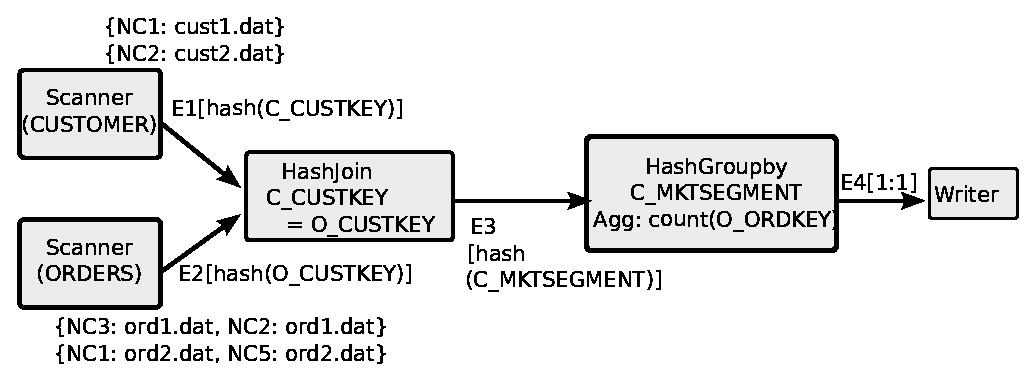
\includegraphics[scale=0.8]{images/tpch-jobspec}
\caption{Example Hyracks job specification}\label{fig:example01_spec}
\end{figure}
\vspace{-2mm}

\vspace{-2mm}
\begin{figure}[htp]
\centering
\includegraphics[scale=0.8]{images/tpch-han}
\caption{Example Hyracks Activity Node graph}\label{fig:example01_han}
\end{figure}
\vspace{-4mm}

\begin{figure*}[htp]
\centering
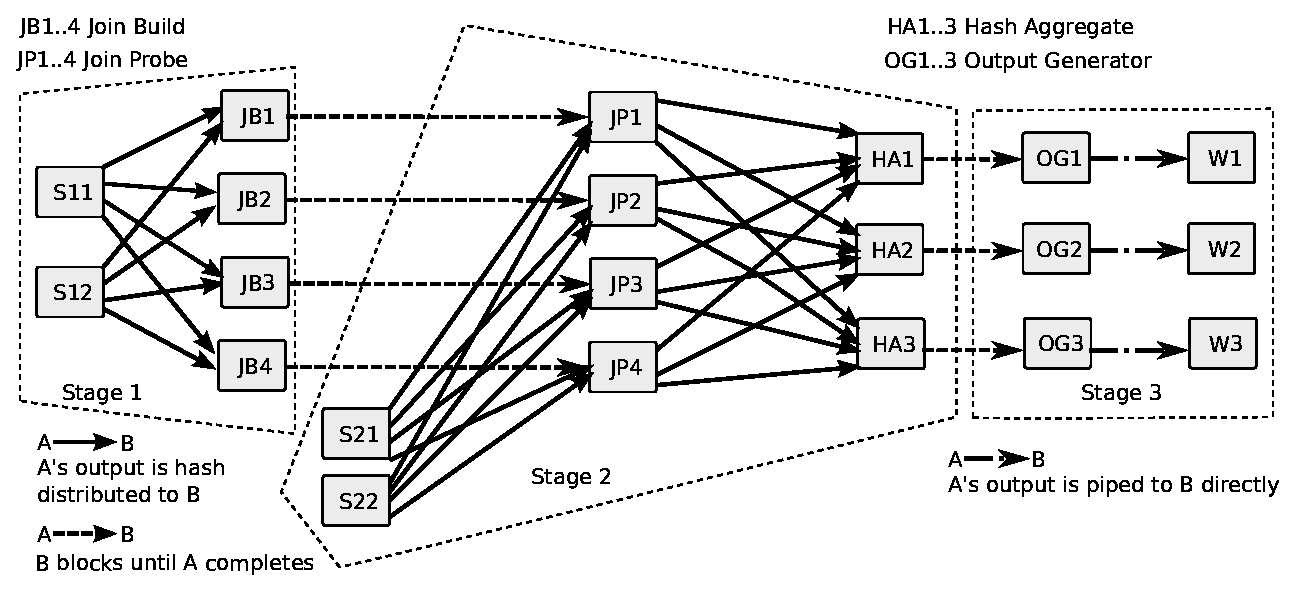
\includegraphics[scale=0.7]{images/tpch-rt}
\caption{Parallel instantiation of the example}\label{fig:example01_rt}
\end{figure*}

\subsection{High-level Architecture}

Figure \ref{fig:sysarch} provides an overview of the basic architecture of a Hyracks installation.
Every Hyracks cluster is managed by a Cluster Controller process.
The Cluster Controller accepts job execution requests from clients, plans their evaluation strategies (e.g., computing stages),
and then schedules the jobs' tasks (stage by stage) to run on selected machines in the cluster.
In addition, it is responsible for monitoring the state of the cluster to keep track of the resource loads at the various worker machines.
The Cluster Controller is also responsible for re-planning and re-executing some or all of the tasks of a job in the event of a failure.
Turning to the task execution side, each worker machine that participates in a Hyracks cluster runs a Node Controller process.
The Node Controller accepts task execution requests from the Cluster Controller and also reports on its health (e.g., resource usage levels)
via a heartbeat mechanism.  More details regarding the controller architecture and its implementation are provided in section \ref{ch:hyracks:sec:implementation}.

\begin{figure}
\centering
\includegraphics[scale=0.8]{images/architecture}
\caption{Hyracks system architecture}\label{fig:sysarch}
\end{figure}

\eat{

Hyracks runs on a shared-nothing cluster of commodity computers with local CPUs, memory, and disks. Figure \ref{fig:sysarch} shows the high level architecture of Hyracks. Some nodes are designated as ``cluster managers'' and assume the responsibility of coordinating and monitoring ``node managers''. A cluster manager is responsible for accepting job creation requests from clients, breaking a job up into discrete stages, deciding parallelization and placement of operators in each stage on the cluster, and initiating job distribution to the node managers. In addition to job management, a cluster manager also receives periodic heartbeats and resource utilization metrics from node managers which it uses in job planning and restarting failed stages. Node managers are responsible for accepting job fragments from a cluster manager and executing them using local resources. The part of a job that is deployed on a node manager is called a joblet. A joblet holds a collection of operators that perform computation on that node. Operators may exchange data with other operators on the same node (using in-process communication) or with operators on other nodes (using network communication). Whenever in-process communication can be used, Hyracks does so without the overhead of data serialization and deserialization. Periodically, node managers send heartbeat messages to cluster managers to show liveness and to relay resource utilization on the node (e.g., CPU, memory and disk activity).

\section{Hyracks jobs}

Clients specify Hyracks jobs as Hyracks Operator Descriptor nodes (HODs) connected to each other by Hyracks Connector Descriptors (HCDs) to form an acyclic directed graph. A HOD node is similar to an execution plan tree node as described in \cite{University97parallelquery}. On receiving such a job specification, the cluster manager first replaces every HOD with one or more Hyracks Activity Nodes (HAN). The process of creating a set of HANs for a HOD are delegated by Hyracks to the HOD object. This allows for an extensible operator framework.

\begin{figure}
\centering
\includegraphics[scale=0.23]{example01}
\caption{Example Hyracks job specification}\label{fig:example01_spec}
\end{figure}

Figure \ref{fig:example01_spec} shows an example specification of a job that computes the total time spent by visitors on a web site. The job gets its inputs from two logical sources called ``visits'' and ``urls''. Let us assume that ``visits'' contains (userid, page\_url, time\_spent) triplets and ``urls'' contains (page\_url, web\_site) pairs. To compute the total time spent by visitors on a website, the two inputs are joined on the ``page\_url'' fields. The output of the join is grouped on the ``web\_site'' field, and finally the ``total\_time'' field is summed up for each group. FS1 and FS2 in the figure are file scanner HODs that are parameterized with the location information of their inputs. As shown, FS1 gets its input in the form of two partitions. The first partition is replicated on the Hyracks node called NC1 in a file called visits1.dat and on NC5 in a file called vis1.dat. The second partition is available only at NC2 in a file called visits2.dat. Similarly, FS2 is configured with an input that is partitioned two ways. The two scanners feed their outputs to a Join HOD. The Join HOD in this example uses the hash-join algorithm. A sorter HOD is used to sort the join output on the web\_site field so that the grouping HOD can operate in constant space. Finally, the file writer HOD is used to produce the result.

Edges in a job specification are annotated with the type of data distribution to use. For example, E1 and E2 use a hash-based distribution on page\_url to distribute the file data to the join instances, routing data from the two sides that match on the page\_url field to the same join operator instance. Similarly, a hash distribution is used by E3 to partition data among the sorters on the web\_site field. E4 is a 1-1 edge that pipes the output of one producer to one consumer. Finally, E5 is an N-1 edge that merges the outputs of the aggregators into the file writer instance.

Figure \ref{fig:example01_han} shows the result of expansion of the HOD graph into the HAN graph. Notice that the original join HOD has been replaced with two activity nodes -- one to perform the build phase of the hash table for the hash-join, and the other to perform the probe on the hash table. A dotted arrow from the builder to the probe indicates a constraint that the probe cannot begin until the builder has completed. Hyracks guarantees that all activity nodes derived from the same HOD are co-located on the same Hyracks node at runtime so they can share information (e.g., the hash table for the join and the run files for the sorter). Note that the two inputs of the original join HOD are now connected to the HANs that actually use them. Similarly, the sort HOD has been replaced with run generation and merging activity nodes.

\begin{figure}
\centering
\includegraphics[scale=0.20]{example01_han}
\caption{Example Hyracks Activity Node graph}\label{fig:example01_han}
\end{figure}

The next step in job planning is to split it into stages. All HANs that are connected only by non-blocking edges are grouped into a stage, splitting the complete job into independent stages. The stages are planned and executed by Hyracks in such a way that all of a stage's dependencies are complete before it is executed. Hyracks plans each stage in order to decide how many instances to create (and where) for each HAN in the stage. To aid this decision, Hyracks asks HANs for any node affinities (e.g., the file scanner must indicate that it should be instantiated where some replica of each partition of the file can be accessed). The job specification can also include constraints regarding the degree of partitioned parallelism of each operator. In addition, Hyracks provides the stage planner with the ability to gather statistics (if any) from preceding stages and use them for planning. Once each stage is planned, the HAN instances are instantiated in participating Hyracks node managers to form a DAG of Hyracks Operator Nodes (HONs) at runtime. Note that the step of planning the degree of parallelism and placement of HONs is delayed until the stage is ready to run -- this allows current cluster conditions (maintained by the Resource Accountant) to play a role in the process. The HONs are responsible for consuming data from their inputs, performing computation, and sending outputs to their consuming HONs. Figure \ref{fig:example01_rt} shows the HON graph for the example. The dotted polygons bound the HONs that form a stage.

\begin{figure*}
\centering
\includegraphics[scale=0.24]{example01_rt}
\caption{Parallel instantiation of the example}\label{fig:example01_rt}
\end{figure*}

}


\section{Computational Model}
\label{ch:hyracks:sec:model}

\eat{

Computational model (3 columns)
    End user model (People, Programs) (1 Figure)
        Hyracks User model (1/2 column)
        Map-Reduce User Model (Compat layer) (1/2 column)
            Describe the TPC-H query as Map/Reduce tasks (1 Figure)
    Operator Implementor Model
        Operator Descriptor
        Operator Activity
        Operator Task
        Connector Descriptor


}

In this section, we describe the Hyracks approach to data representation and the Hyracks programming model as they pertain to two broad classes of users:
end users who use Hyracks as a Job assembly layer to solve problems, and operator implementors who wish to implement new operators for use by end users.
(Compilers for higher-level languages essentially fall into the first class of users as well.)
We also describe the built-in operators and connectors that are available as part of the initial software distribution of Hyracks.

\subsection{Data Treatment in Hyracks}

In Hyracks, data flows between operators over connectors in the form of records that can have an arbitrary number of fields.
Hyracks provides support for expressing data-type-specific operations such as comparisons and hash functions.
The type of each field is described by providing an implementation of a descriptor interface that allows Hyracks to perform serialization and deserialization.
For most basic types, e.g., numbers and text, the Hyracks library contains pre-existing type descriptors.
The Hyracks use of a record as the carrier of data is a generalization of the (key, value) concept found in MapReduce and Hadoop.
The advantage of the generalization is that operators do not have to artificially package (and repackage) multiple data objects into a single ``key'' or ``value'' object \footnote{It is interesting to note that Apache Flink (previously known as Nephele/PACTS) switched to this model from the key-value model recently.}.
The use of multiple fields for sorting or hashing also becomes natural in this model.
For example, the Hyracks operator library includes an external sort operator descriptor
that can be parameterized with the fields to use for sorting along with the comparison functions to use.
Type descriptors in Hyracks are similar to the Writable and WritableComparator interfaces in Hadoop.
However, a subtle but important difference is that Hyracks does not require the object instances that flow between operators to themselves implement a specific interface;
this allows Hyracks to directly process data that is produced and/or consumed by systems with no knowledge of the Hyracks platform or its interfaces.

\subsection{End User Model}

Hyracks has been designed with the goal of being a runtime platform
where users can hand-create jobs, like in Hadoop and MapReduce, yet at
the same time to be an efficient target for the compilers of
higher-level programming languages such as Pig, Hive, or Jaql. In
fact, the Hyracks effort was born out of the need to create an
appropriate runtime system for the ASTERIX project at UCI
\cite{asterix:website}, a project in which we are building a scalable
information management system with support for the storage, querying,
and analysis of very large collections of semi-structured nested data
objects using a new declarative query language (AQL).
Figure~\ref{fig:enduser} shows the entire AsterixDB stack.

\subsubsection{Hyracks Native User Model}

A Hyracks job is formally expressed as a DAG of operator descriptors
connected to one another by connector descriptors, as was indicated in
Figure \ref{fig:example01_spec}.  In addition to its input and output
connectors, an operator descriptor may take other parameters specific
to its operation.  For example, the ExternalSortOperatorDescriptor in
the Hyracks built-in operator library needs to know which fields in
its input record type are to be used for sorting, the comparators to
use to perform the sorting operation, and the amount of main memory
budgeted for its sorting work.

Hyracks currently allows users to choose between two ways of
describing the scheduling choices for each of the operators in a job.
One option is to list the exact number of partitions of an operator to
be created at runtime along with a list of choices of worker machines
for each partition.  Another option is just to specify the number of
partitions to use for an operator, leaving Hyracks to decide the
location assignments for each of its partitions.

\begin{figure} [htb!]
  \centering
  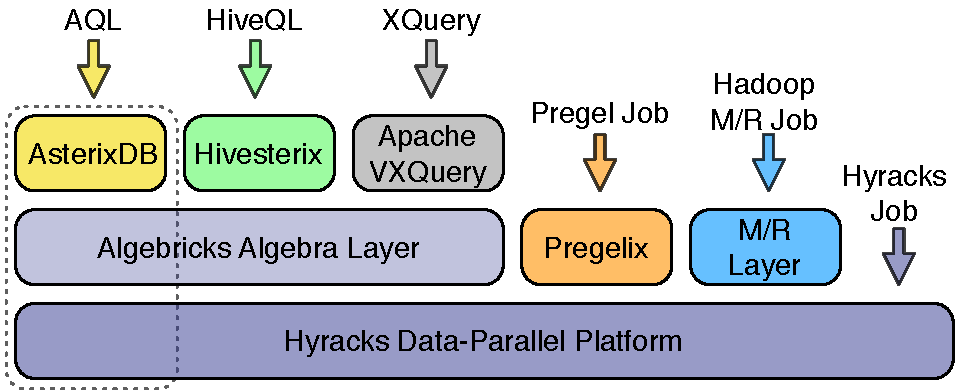
\includegraphics[width=6in]{images/asterixdb_stack}
  \caption{End User Models of Hyracks}
  \label{fig:enduser}
\end{figure}

\subsubsection{Hyracks Map-Reduce User Model}

MapReduce has become a popular paradigm for data-intensive parallel computation using shared-nothing clusters.
Classic example applications for the MapReduce paradigm have included processing and indexing crawled Web documents, analyzing Web request logs, and so on.
In the open source community, Hadoop is a popular implementation of the MapReduce paradigm that is quickly gaining traction even in more traditional enterprise IT settings.
To facilitate easy migration for Hadoop users who wish to use Hyracks, we have built a Hadoop compatibility layer on top of Hyracks.
The aim of the Hyracks Hadoop compatibility layer is to accept Hadoop jobs unmodified and run them on a Hyracks cluster.

In MapReduce and Hadoop, data is initially partitioned across the nodes of a cluster and stored in a distributed file system (DFS).
Data is represented as \texttt{(key, value)} pairs.
The desired computation is expressed using two functions:
\begin{alltt}
map    (k1,v1)       \(\rightarrow\) list(k2,v2);
reduce (k2,list(v2)) \(\rightarrow\) list(k3,v3).
\end{alltt}

A MapReduce computation starts with a map phase in which the \texttt{map} functions are applied in parallel on different partitions of the input data.
The \texttt{(key, value)} pairs output by each \texttt{map} function are then hash-partitioned on their \texttt{key}.
For each partition, the pairs are sorted by their \texttt{key} and sent across the cluster in a shuffle phase.
At each receiving node, all of the received partitions are merged in sorted order by their \texttt{key}.
All of the pair values sharing a given key are then passed to a single reduce call.
The output of each \texttt{reduce} function is finally written to a distributed file in the DFS.

To allow users to run MapReduce jobs developed for Hadoop on Hyracks, we developed two extra operator descriptors that can wrap the
\texttt{map} and \texttt{reduce} functionality.\footnote{The \texttt{combine} functionality of MapReduce is fully supported as well,
but those details are omitted here for ease of exposition.} 
The data tuples provided as input to the \id{hadoop\_mapper} operator descriptor are treated as \texttt{(key, value)} pairs and,
one at a time, passed to the \texttt{map} function.
The \id{hadoop\_reducer} operator descriptor also treats the input as \texttt{(key, value)} pairs, and groups the pairs by \texttt{key}.
The sets of \texttt{(key, value)} pairs that share the same \texttt{key} are passed, one set at a time, to the \texttt{reduce} function.
The outputs of the \texttt{map} and \texttt{reduce} functions are directly output by the operator descriptors.
To emulate a MapReduce framework we employ a sort operator descriptor and a hash-based distributing connector descriptor.

\begin{figure*}[!htb]
\centering

\includegraphics[scale=0.7]{images/hyrax-hadoop}
\caption{Hyracks plan for Hadoop jobs}\label{fig:hyrax-hadoop}
\end{figure*}

Figure~\ref{fig:hyrax-hadoop} shows the Hyracks plan for running a MapReduce job.
After data is read by the scan operator descriptor, it is fed into the \id{hadoop\_mapper} operator descriptor using a 1:1 edge.
Next, using an $M$:$N$ hash-based distribution edge, data is partitioned based on \texttt{key}.
(The ``$M$'' value represents the number of maps, while the ``$N$'' value represents the number of reducers.)
 After distribution, data is sorted using the sort operator descriptor and passed to the \id{hadoop\_reducer} operator descriptor using a 1:1 edge.
Finally, the \id{hadoop\_reducer} operator descriptor is connected using a 1:1 edge to a file-writer operator descriptor.

\subsection{Operator Implementor Model}

One of the initial design goals of Hyracks has been for it to be an extensible runtime platform.
To this end, Hyracks includes a rich API for operator implementors to use when building new operators.
The implementations of operators made available ``out of the box'' via the Hyracks operator library are also based on the use of this same API.

Operators in Hyracks have a three-part specification:
\begin{enumerate}
\item \emph{Operator Descriptors}: Every operator is constructed as an implementation of the Operator Descriptor interface.
Using an operator in a job involves creating an instance of the descriptor of that operator.
The descriptor is responsible for accepting and verifying parameters required for correct operation from the user during job assembly.
During the job planning phase, the descriptor is responsible for expanding itself into its constituent activities (as illustrated back in Figure~\ref{fig:example01_han}).
\item \emph{Operator Activities}: Hyracks allows an operator to describe, at a high level, the various phases involved in its evaluation.
Phases in an operator usually create sequencing dependencies that describe the order in which the inputs of the operator
are required to be made available and the order in which the outputs will become available.
Again, Figure \ref{fig:example01_han} showed the expansions for the hash-join and the hash-based grouping operators into their component activities.
As a part of the expansion, activities indicate any blocking dependencies and the mapping of overall operator inputs and outputs to the activities' inputs and outputs.
For example, when the hash-join operator is expanded, it indicates to Hyracks that its join-build activity consumes one input and its join-probe activity consumes the other.
It also indicates that its join-probe activity produces the output.
At a high level, this describes to Hyracks that the second input is not required to be available until the stage containing the join-build activity is complete.
Conversely, it also indicates that output from the join will not be available until the stage containing the join-build activity is complete.
Hyracks then uses this information to plan the stages of a job in order of necessity.
Deferring planning to the moment just prior to execution allows Hyracks to use current cluster conditions
(availability of machines, resource availability at the various machines, etc.) to help determine the schedule for a stage's tasks.
\item \emph{Operator Tasks}: Each activity of an operator actually represents a \emph{set} of parallel tasks to be scheduled on the machines in the cluster.
Tasks are responsible for the runtime aspect of the activity -- each one consumes a partition of the activity's inputs and produces a partition of its output.
The tasks corresponding to activities of the same partition of the same operator may need to share state.
For example, the join-probe task needs to be given a handle to the hashtable constructed by the join-build task.
To facilitate such state sharing, Hyracks co-locates those tasks that belong to a given partition of an activity of the same operator.
For example, in Figure \ref{fig:example01_rt}, the join-probe tasks are co-located with their corresponding join-build tasks.
Note that the join-build task will no longer be active when the join-probe task is scheduled, but Hyracks provides a shared context
for the two tasks to use to exchange the required information.
In the future we plan to explore alternative state transfer mechanisms (albeit at a higher cost),
e.g., to use when co-location is impossible due to resource constraint violations at a machine.
In terms of operator implementation, the implementor of a new operator can implement the runtime behavior
of its activities by providing single-threaded implementations of an iterator interface (a la \cite{GraefeQP}),
much as in Gamma \cite{GammaTKDE}.

\subsection{Hyracks Library}

Hyracks strongly promotes the construction of reusable operators and connectors that end users can then just use to assemble their jobs.
Hyracks, as part of its software distribution, comes with a library of pre-existing operators and connectors.
Here we briefly describe some of the more important operators and connectors.

\subsubsection{Operators}

\begin{asparaitem}
\item \emph{File Readers/Writers}:
\begin{asparaitem}
\item \emph{Line File Reader/Writer}: Reads/writes files from/to the local file system, treating a file as a sequence of lines.
\item \emph{Delimited File Reader/Writer}: Reads/writes files from/to the local file system; the files contain records separated by record delimiters,
and the records contain fields separated by field delimiters. %% The operator can be parameterized to configure its delimiters.
\item \emph{HDFS File Reader/Writer}: Reads/writes files from/to the Hadoop Distributed File system. %% The input format of the file being read/written can be configured.
%% These operators are used by the Hadoop compatibility layer to read/write files from/to HDFS, but they can also be used in the assembly of arbitrary Hyracks jobs.
\end{asparaitem}
\item \emph{Mappers}:
\begin{asparaitem}
\item \emph{Native mapper}: Used to evaluate a function once for each item in the input. Mappers can be used to implement traditional operators such
as projection and selection. %% from the relational algebra. 
%% The Mapper operator is parameterized with the function to be called for each item in its input.
\item \emph{Hadoop Mapper}: Used to call the Mapper interface in the Hadoop MapReduce library.
It is used by the compatibility layer to invoke Hadoop mappers.
\end{asparaitem}
\item \emph{Sorters}:
\begin{asparaitem}
\item \emph{In-memory Sorter}: Uses main memory to sort its input. 
% It accepts the fields in the input to use along with the comparators for those fields
% to sort the input data.
\item \emph{External Sorter}: Tries to use a main memory allocation to sort its input data, but when the input does not fit into memory,
it creates and merges runs on disk. %% It accepts the fields in the input to use along with the comparators for those fields to sort the input data (like
%% the in-memory sorter). It also accepts the maximum memory budget available for its use.
\end{asparaitem}
\item \emph{Joiners}:
\begin{asparaitem}
\item \emph{In-memory Hash Joiner}: Performs an equijoin by using memory to build a hash-table on one input and then probing the table with the other input.
%% It accepts the set of fields from each side that have to match for the join. In addition, it accepts the hash-functions to use to build and probe the hashtable and the
%% comparators to to compare the field values.
\item \emph{Hybrid Hash Joiner}: Performs an equijoin using the hybrid hash-join algorithm \cite{GraefeQP}. 
% It works with bounded memory by creating overflow partitions
% when the input data is larger than its provided memory budget. In addition to the parameters required by the In-memory Hash Joiner, it also accepts a memory budget.
\item \emph{Grace Hash Joiner}: Performs an equijoin using the Grace hash-join algorithm \cite{GraefeQP}. 
% It works with bounded memory by eagerly partitioning each input
% and then performing in-memory hash joins of the corresponding partitions of each input one-at-a-time. It requires the same parameters as the Hybrid Hash Joiner.
\end{asparaitem}
\item \emph{Aggregators}:
\begin{asparaitem}
\item \emph{Hash-based Aggregator}: Groups input data using an in-memory hash table. A custom aggregator function is invoked for each group of the input data.
%% The operator accepts the fields to use for grouping along with the hash-functions and the comparators for those fields.
\item \emph{Preclustered Aggregator}: Groups input data using very little state assuming it is already clustered on the grouping fields.
%% Similar to the hash-based aggregator, it invokes a custom aggregator function for each group.
% This operator can be used if during job assembly it is known that the input data to this operator satisfies the clustered property.
% Alternatively, one of the Sorter operators can be used to enforce this data property prior to aggregation.
\end{asparaitem}
\end{asparaitem}

\subsubsection{Connectors}
Connectors distribute data produced by a set of \emph{sender}
operators to a set of \emph{receiver} operators.
\begin{asparaitem}
\item \emph{M:N Hash-Partitioner:} Hashes every tuple produced by
  senders (on a specified set of fields) to generate the receiver
  number to which the tuple is sent.  Tuples produced by the same
  sender keep their initial order on the receiver side.
% , but there is
%   no guarantee regarding the order of tuples coming from different
%   senders.
\item \emph{M:N Hash-Partitioning Merger:} Takes as input sorted
  streams of data and hashes each tuple to find the receiver. On
  the receiver side, it merges streams coming from different senders
  based on a given comparator, thus producing ordered partitions.
\item \emph{M:N Range-Partitioner:} Takes the position $k$ of the
  partitioning field and a set of disjoint $n$ ranges, each range
  associated with one of the $n$ receiver operators. (The field at
  position $k$ must always contain integer values.) Every tuple
  produced by a sender is distributed to the receiver associated
  with the range in which the value of the $k$-th field lies.
\item \emph{M:N Replicator:} Copies the data produced by every sender
  to every receiver operator.
\item \emph{1:1 Connector:} Connects exactly one sender to one receiver
  operator. % , sending all data from the output of the sender to the input
%   of the receiver.

\end{asparaitem}

\end{enumerate}


\section{Hyracks Implementation details}
\label{ch:hyracks:sec:implementation}

In this section we describe some of the details of the Hyracks implementation.
We first describe the control portion of Hyracks, which maintains cluster membership and performs job scheduling, tracking, and recovery.
We then discuss some of the salient implementation details of modules that help Hyracks to run its operators and connectors efficiently.

\subsection{Control Layer}
\label{ch:hyracks:sec:implementation:subsec:control}

As was shown in Figure \ref{fig:sysarch}, a Cluster Controller (CC) is used to manage a Hyracks cluster.
Worker machines are added to a Hyracks cluster by starting a Node Controller (NC) process on that machine and
providing it with the network address of the Cluster Controller process whose cluster it is to join. The NC then initiates
contact with the CC and requests registration.
As part of its registration request, the NC sends details about the resource capabilities (number of cores, etc.) of its worker machine.
On successful registration, the CC replies to the NC with the rate at which the NC should provide heartbeats back to the CC to maintain continued membership in the cluster.

On receiving a job submission from a client, the CC infers the stages of the job (as was illustrated in Figures~\ref{fig:example01_han} and~\ref{fig:example01_rt}). Scheduling of a stage that is ready
to execute is performed using the latest information available about the cluster. (This may happen much later than when the job was submitted, e.g., in a long multi-stage job.)
Once it has determined the worker nodes that will participate in the execution of the stage, the CC initiates task activation on those worker nodes in parallel by pushing a
message to start the tasks. This is different from the way the Hadoop Job Tracker disseminates tasks to the Task Trackers -- Hadoop uses a pull model where the Task Trackers pull
tasks from the Job Tracker by means of a periodic heartbeat.
Although eagerly pushing job start messages increases the number of messages on the cluster, we have adopted this approach to minimize the wait time for tasks to start execution.
This becomes increasingly important as a platform tries to target short jobs.
In the future, we will explore ways of minimizing the network traffic for control messages by exploiting opportunities to piggyback multiple messages targeting the same NC.

The control logic of the Hyracks Cluster Controller was initially implemented in Overlog \cite{BOOM} using the JOL~\cite{jol:website} library. It was later reimplemented in Java due to performance concerns. We describe the Overlog implementation here since it provides insight into the behavior of the control layer in Hyracks.

Overlog is an extension of Datalog that has support
for events. Integration with JOL was convenient since both JOL and Hyracks are implemented in Java. The JOL implementation of Overlog models data as tables of records with
a declared schema. The fields in the tables can be arbitrary Java objects. JOL allows
Java code to register callbacks that are invoked by the Overlog interpreter when modifications are made to the tables. JOL also allows insertion and deletion of records
in a table from Java. At a very high level, the Java code in the CC is used to translate events from the outside world (clients submitting jobs and NC registrations/heartbeats)
into inserts and deletes on JOL tables. This action triggers the JOL interpreter to execute the JOL program which results in modifications to one or more tables that have
Java callbacks attached. When invoked with data that is inserted into or deleted from the tables by JOL, these callbacks apply the desired effects in the outside world
(e.g., by sending start/abort task messages to the NCs). Figure~\ref{fig:jolcontroller} shows the role of JOL and Java code as a controller framework.

\vspace{-1mm}
\begin{figure} [htb!]
  \centering
  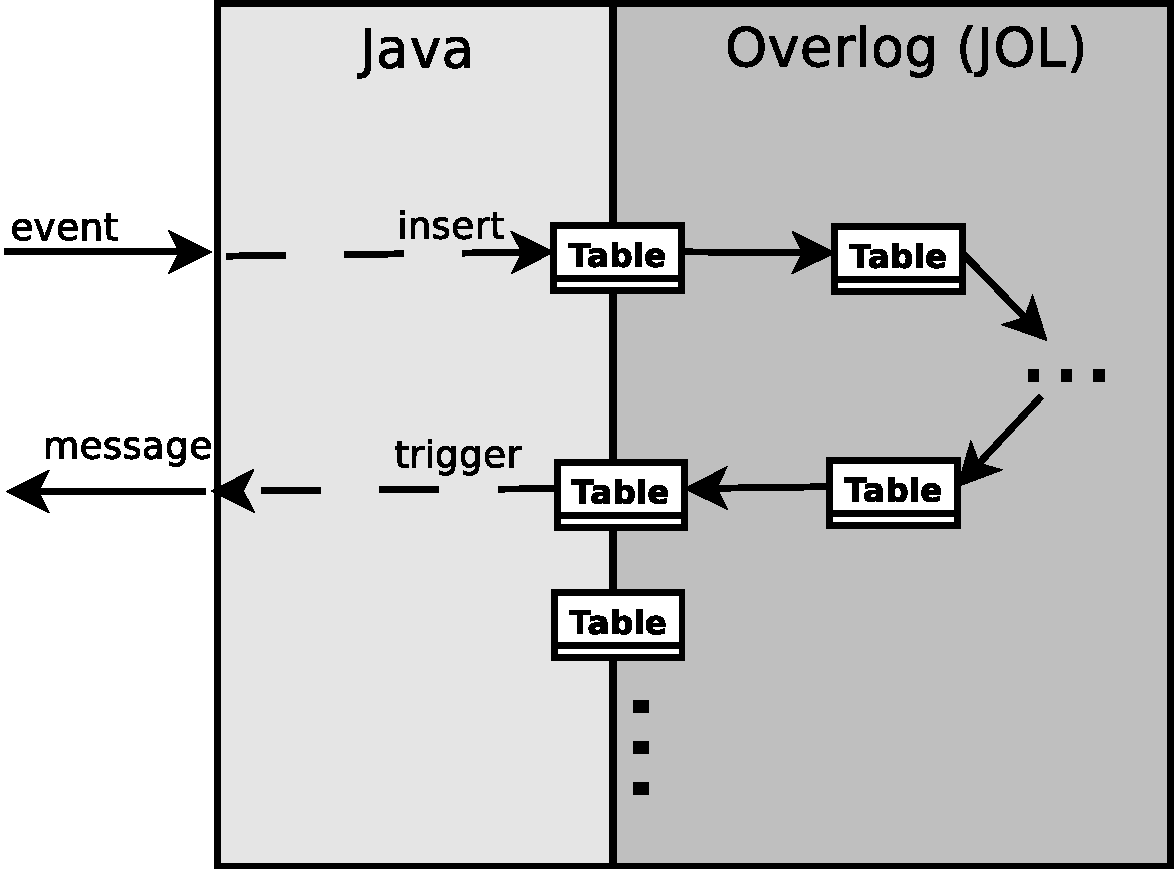
\includegraphics[scale=0.5]{images/jolcontroller}
  \caption{Mixed Java/JOL controller framework}
  \label{fig:jolcontroller}
\end{figure}
\vspace{-1mm}

Table~\ref{tbl:joltables} shows a few of the JOL tables that are relevant to identifying the stages of a Hyracks job. When a job is submitted, the CC translates the
job specification into insertions of records into the \id{operatordescriptor} (one record per Operator Descriptor) and \id{connectordescriptor} (one record per Connector
Descriptor) tables. It then visits every Operator Descriptor in the job specification and inserts a record into the \id{activitynode} table for every activity of each Operator
Descriptor. As part of the expansion of the Operator Descriptor into activities, a mapping from the Operator Descriptor inputs (and outputs) to the Operator Task inputs (and
outputs) is provided along with blocking dependencies between activities. The input/output mapping is captured in the \id{activityconnection} table while the blocking information
is captured in the \id{activityblocked} table. Once the CC has inserted records into these tables, it invokes the JOL runtime to evaluate the Overlog program.
Figure~\ref{fig:jolcontroller} shows the part of the Overlog program used by the Cluster Controller to infer stages of activities and populate the \id{activitystage\_rec} and
\id{activitystage} tables. The \id{activitystage\_rec} table is populated using rules 1 thru 4 recursively and the final result of stage assignments to activities is recorded
in the \id{activitystage} table. The rules specified in Overlog can be summarized as follows:
\begin{enumerate}
\item Rule 1: Initially assume all activities can be evaluated in the earliest stage by inserting an assignment of stage 0 to every activity in the \id{activitynode} table.
\item Rule 2: If an activity A1 must block on activity A2, and A1 is assigned a stage earlier than or the same as A2, insert a stage assignment for A1 that is one greater
than the stage assigned to A2.
\item Rules 3 and 4: If activity A1 is connected to activity A2 through a Connector Descriptor, and A1 and A2 belong to different stages, insert a stage assignment for A1 that
is the later of A1's and A2's stages. This rule occurs twice, once for A1 and once for A2, because the \id{connectordescriptor} table captures a one-way connection whereas
for the stage assignment we concern ourselves with the existence of a connection. Intuitively, if we wish to co-schedule (for pipelining) the activities connected by a data
flow connector, they will both need to be assigned to the latter of the stages to which they belong.
\item Rule 5: Finally, the actual stage number associated with an activity is the maximum over all of the stage number assignments and is captured in the \id{activitystage} table.
\end{enumerate}

\begin{table*}
\center
\caption{Tables identifying stages of a Hyracks job.}\label{tbl:joltables}
\begin{footnotesize}
\begin{tabular}{|l|l|}
\hline
Table Name & Table Attributes \\
\hline \hline
\id{operatordescriptor} & JobId, OperatorDescriptorId, OperatorDescriptor  \\
\hline
\id{connectordescriptor} & JobId, ConnectorDescriptorId, SourceOperatorId, \\ & SourcePort, TargetOperatorId, TargetPort, ConnectorDescriptor \\
\hline
\id{activitynode} & JobId, OperatorDescriptorId, ActivityId, Activity \\
\hline
\id{activityconnection} & JobId, OperatorDescriptorId, OperatorPort, \\ & Direction, ActivityId, ActivityPort \\
\hline
\id{activitystage} & JobId, OperatorDescriptorId, ActivityId, StageNumber \\
\hline
\id{activityblocked} & JobId, BlockingOperatorDescriptorId, BlockingActivityId, \\ & BlockedOperatorDescriptorId, BlockedActivityId \\
\hline
\end{tabular}
\end{footnotesize}
\end{table*}

\eat{
\begin{table*}
\caption{Fragment of Overlog program for inferring stages of activities.}
\label{fig:jolexample}
\begin{footnotesize}
\begin{tabular}{|l|l|l}
activitystage\_rec & (JobId, OpId, ActivityId, 0) \pdef 
     activitynode(JobId, OpId, ActivityId,\longunderscore); & (1)\\
activitystage\_rec & (JobId, OpId2, ActivityId2, Stage) \pdef 
     activitystage\_rec(JobId, OpId1, ActivityId1, Stage1), & (2) \\
&     activitystage\_rec(JobId, OpId2, ActivityId2, Stage2),\\
&     activityblocked(JobId, OpId1, ActivityId1, OpId2, ActivityId2), \\
&     Stage2 \leq Stage1 \ \ \{\ \ Stage := Stage1 + 1;\ \  \}; \\
activitystage\_rec & (JobId, OpId2, ActivityId2, Stage) \pdef 
    activitystage\_rec(JobId, OpId1, ActivityId1, Stage1), & (3) \\
  &  activitystage\_rec(JobId, OpId2, ActivityId2, Stage2), \\
  &  activityconnection(JobId, OpId1, Op1Port, Dir.OUT, ActivityId1, \longunderscore), \\
  &  activityconnection(JobId, OpId2, Op2Port, Dir.IN, ActivityId2, \longunderscore), \\
  &  connectordescriptor(JobId, \longunderscore\,,, OpId1, Op1Port, OpId2, Op2Port, \longunderscore), \\
  &  Stage1 \neq  Stage2 \ \  \{\ \ Stage := java.lang.Math.max(Stage1, Stage2);\ \ \}; \\
activitystage\_rec & (JobId, OpId1, ActivityId1, Stage) \pdef 
     activitystage\_rec(JobId, OpId1, ActivityId1, Stage1), & (4) \\
   & activitystage\_rec(JobId, OpId2, ActivityId2, Stage2), \\
   & activityconnection(JobId, OpId1, Op1Port, Dir.OUT, ActivityId1, \longunderscore), \\
   & activityconnection(JobId, OpId2, Op2Port, Dir.IN, ActivityId2, \longunderscore), \\
   & connectordescriptor(JobId,\longunderscore\,, OpId1, Op1Port, OpId2, Op2Port, \longunderscore), \\
   &  Stage1 \neq  Stage2 \ \  \{\ \ Stage := java.lang.Math.max(Stage1, Stage2);\ \ \}; \\
activitystage & (JobId, OpId, ActivityId, max<Stage>) %\pdef 
     activitystage\_rec(JobId, OpId, ActivityId, Stage); & (5)
\end{tabular}
\end{footnotesize}
\end{table*}
}
The scheduling and fault-recovery logic was also implemented in Overlog using the general principles described above. Although Overlog was very expressive and could succinctly represent most logic that was necessary for performing scheduling actions and handling faults, it had some major drawbacks. The simple act of assigning a monotonically increasing integer to each item in a collection, which can be implemented to have linear complexity in any imperative language, is a quadratic operation in Overlog. Assigning such an integer, involves repeatedly computing the maximum number assigned so far, and assigning one more than that number to the ``next'' item in the collection. Quite a few places in the Hyracks control layer needed the assignment of sequential numbers (for example, the assignment of partition ids to the Hyracks Operator Nodes), and the quadratic complexity of this operation created a performance bottleneck when the collection sizes were large. This directly translated to longer scheduling times for large jobs. Since there was no easy way to work around this issue (and it was not our focus, at that time), we decided to reimplement the control layer in Java to recapture all the lost performance in an expedient manner. It would be interesting to investigate ways of adding efficient mechanisms for number assignment to a language like Overlog.

\subsection{Task Execution Layer}

Once a stage of a Hyracks job becomes ready to run,
the CC activates the stage on the set of NCs that have been chosen to run the stage and then waits until the stage completes or until an NC failure is detected.
In the remainder of this section we explore the task activation process and then discuss some details of the implementation of the data-processing and data-movement
aspects of Tasks and Connectors, respectively.

\subsubsection{Task Activation}

When a stage becomes ready to run, the Cluster Controller sends messages to the Node Controllers participating in that stage's execution to perform task activation in three
steps.
\begin{enumerate}
\item \emph{Receiver Activation}: The CC initiates a ReceiverActivation request to every NC that participates in a stage's execution. Each NC, on receipt of this request,
creates the Task objects that have been designated to run at that NC (as determined by the scheduler). For each Task that accepts inputs from other
Tasks, it creates an endpoint that has a unique network address. The mapping from a Task object's input to the endpoint address is relayed back to the CC as the response to
this request.
\item \emph{Sender-Receiver Pairing}: Once the CC receives the ReceiverActivation responses containing local endpoint addresses from the NCs, it merges all of them together to
create a global endpoint address map. This global map is now broadcast to each NC so that the send side of each Task object at that NC knows the network addresses of its
consumer Tasks.
\item \emph{Connection Initiation}: Once pairing has completed on all NCs, the CC informs all of the NCs that the Tasks can be started.
\end{enumerate}

\subsubsection{Task Execution and Data Movement}

The unit of data that is consumed and produced by Hyracks tasks is called a Frame.
A frame is a fixed-size (configurable) chunk of contiguous bytes. A producer of data packs a frame
with a sequence of records in a serialized format and sends it to the consumer who then interprets the records. Frames never contain partial records; in other words, a record
is never split across frames. A naive way to implement tasks that process records is to deserialize them into Java objects and then process them. However, this 
has the potential to create many objects, resulting in more data copies (to create the object representation) and a burden on the garbage collector (later) to reclaim
the space for those objects. To avoid this problem, Hyracks provides interfaces for comparing and hashing fields that can be implemented to work off of the binary data
in a frame. Hyracks includes implementations of these interfaces for the basic Java types (String, integer, float, etc.). Hyracks also provides Task implementors with helper
functions to perform basic tasks on the binary data such as to copy complete records, copy specific fields, and concatenate records from source frames to target frames.

A task's runtime logic is implemented as a push-based iterator that receives a frame at a time from its inputs and pushes result frames to its consumers. Note that the task-runtime only
implements the logic to process streams of frames belonging to one partition without regards to any repartitioning of the inputs or outputs that might be required. Any
repartitioning is achieved by using a Connector. The connector runtime has two sides, the send-side and the receive-side. There are as many send-side instances of a connector
as tasks in the producing activity, while there are as many receive-side instances as tasks in the consuming activity. The send-side instances are co-located with the
corresponding producer tasks, while the receive-side instances are co-located with the consuming tasks. When a send-side instance of a connector receives a frame from its
producing task, it applies its redistribution logic to move records to the relevant receive-side instances of the connector. For example, the M:N hash-partitioning
connector in Hyracks redistributes records based on their hash-value. The send-side instances of this connector inspect each record in the received frame, compute
the hash-value, and copy it to the target frame meant for the appropriate receive-side instance. When a target frame is full, the send-side instance sends the frame to
the receive-side instance. If the send-side and receive-side instances of a connector are on different worker machines (which is most often the case), sending a frame
involves writing it out to the network layer. The network layer in Hyracks is responsible for making sure that the frame gets to its destination.

In order to use network buffers efficiently on the receive-side of a connector, Hyracks allows the connector implementation to specify the buffering strategy for received
frames. Figure~\ref{fig:networkbuffers} shows two buffering strategies that could be chosen by a connector. If the receive-side logic of a connector does not differentiate
between the frames sent by the various send-side instances, it can choose to use one network buffer for all senders. On the other hand, if the connector's logic requires
treating frames from different senders separately, it can use one network buffer per send-side instance. For example, the M:N hash-partitioning connector does not differentiate
frames based on their senders. However, an M:N sort-merge connector, which assumes that frames sent by a sender contain records that are pre-sorted, needs to decide which
sender's frame to read next in order to perform an effective merge.

\vspace{-1mm}
\begin{figure} [htb!]
  \begin{minipage}[b]{0.38\linewidth}
  \centering
  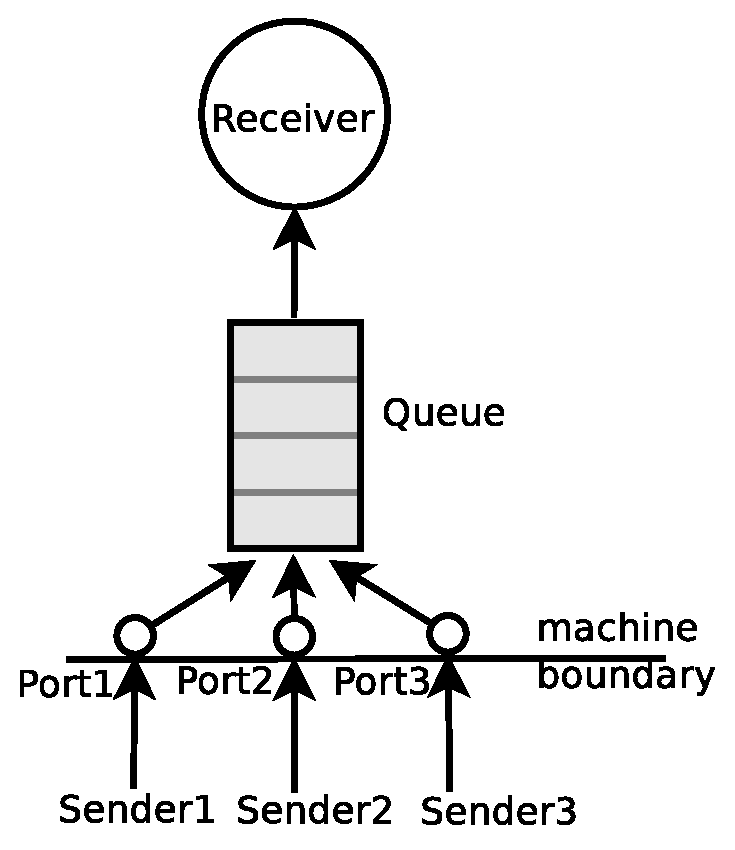
\includegraphics[scale=0.3, trim=10 10 30 10]{images/connector1}
  \legend{Shared buffer}
  \end{minipage}
  \begin{minipage}[b]{0.55\linewidth}
  \centering
  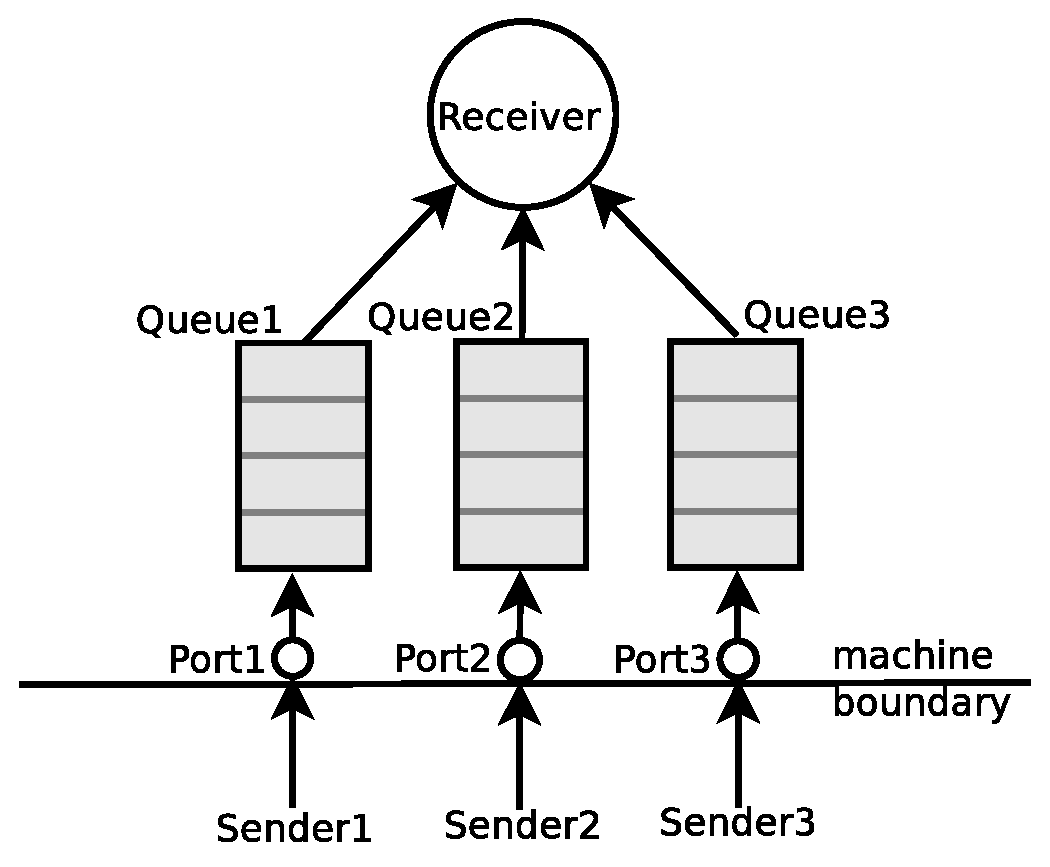
\includegraphics[scale=0.3, trim=7 10 40 10]{images/connector2}
  \legend{One buffer per sender}
  \label{subfig:networkbuffers}
  \end{minipage}
  \caption{Buffering strategies for connectors.}\label{fig:networkbuffers}
\end{figure}
\vspace{-1mm}

\section{Experimental Results}
\label{ch:hyracks:sec:experiments}

In this section we report the results of early performance comparisons (erformed in 2011) of Hadoop and Hyracks as data-intensive computing platforms. First, we compare the performance
of jobs written using the
MapReduce paradigm by running them on Hadoop and running the same jobs unchanged on Hyracks using its Hadoop compatibility layer. Next, we show the difference in performance
that results from not being limited to the MapReduce model in Hyracks. Finally, we explore the performance of Hadoop and Hyracks when node failures occur by using a simple model
for generating failures.

For all of the experiments shown in this section, we used a cluster
of ten IBM machines each with a 4-core Xeon 2.27 GHz CPU, 12GB of main memory, and four locally attached 10,000 rpm SATA drives. The same cluster was used for Hyracks
as well as Hadoop. The Hadoop version used was 0.20.1 (the latest release available when these experiments were performed, in 2011).

\subsection{MapReduce on Hyracks}

In this section, we compare the running times of three very different kinds of jobs (K-Means clustering, a TPC-H style query, and Set-Similarity Joins) on Hadoop
versus on Hyracks using the compatibility layer.

\subsubsection{K-Means}
K-Means is a well known clustering algorithm that tries to find clusters given a set of points. Mahout \cite{mahout:website} is a popular open source project
that includes a Hadoop implementation of the K-Means algorithm as MapReduce jobs.
The clustering problem
consists of grouping a set of $n$ points into $k$ clusters
$\{C_i\}_{i=1,k}$ with centers $\{\mu_i\}_{i=1,k}$, such that each
point is assigned to the cluster with the closest center. The K-Means
MapReduce implementation~\cite{nips06-mapreducemulticore} starts with a randomized
algorithm (called canopy computation) to heuristically determine the number of
clusters that the K-Means algorithm must try to find.
The canopy MapReduce job finds $k$ points to serve as initial centroids of the
$k$ clusters that will then be refined by subsequent iterations of the K-Means algorithm.
Each iteration of the K-Means algorithm is also implemented as a MapReduce job. The Map phase
scans over the set of data points in the input and finds their closest centroid $\mu_j$ among
the $k$ centroids computed in the previous step. Once the closest centroid is found,
that input point is deemed to belong to cluster $j$. The output of the Map phase is
regrouped by the cluster assignment of each point and routed to the Reducers.
The Reduce phase computes a new cluster centroid for each of the $k$ clusters by averaging the coordinates of all points assigned to that cluster.

\begin{figure} [htb!]
  \centering
  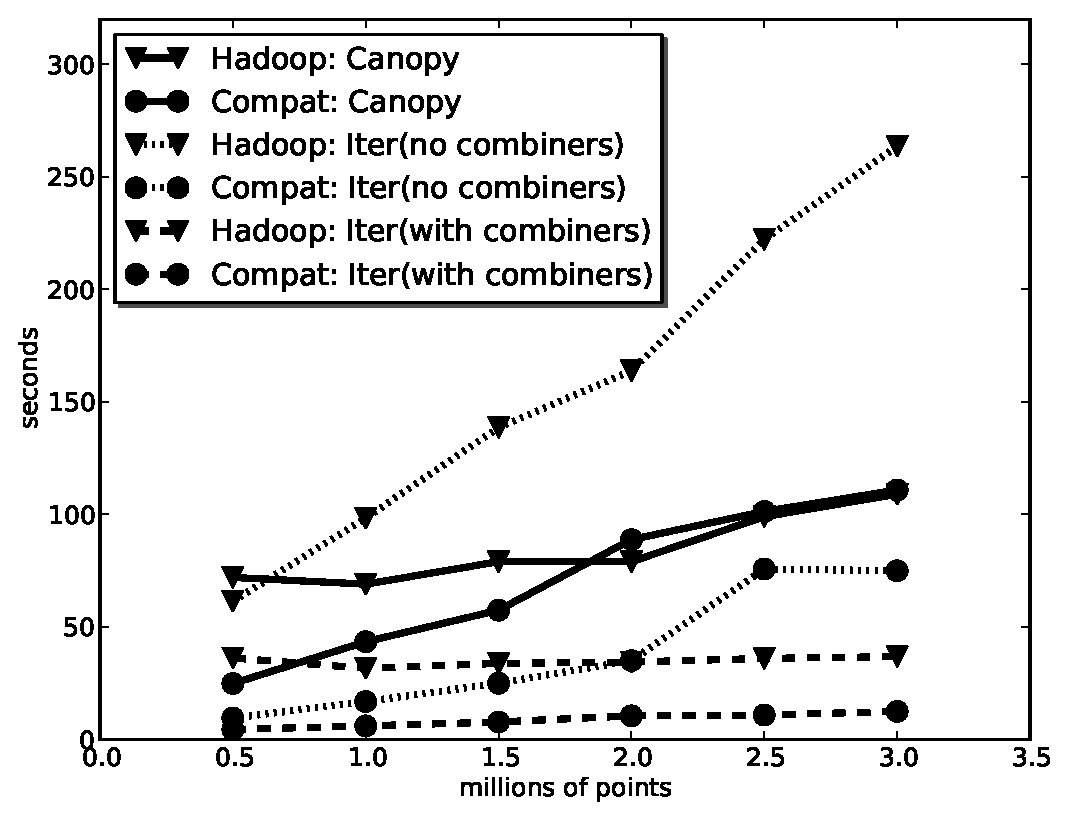
\includegraphics[scale=0.6]{images/KMeans}
  \caption{K-Means on Hadoop and Hyracks}
  \label{fig:kmeans}
\end{figure}

In Figure~\ref{fig:kmeans} we show separately the time taken by the canopy computation
phase and by the iterations for K-Means on both systems. We further explore the efficiency tradeoffs
of Hyracks vs. Hadoop as a data-platform by presenting the average running-time of the iterations both with and
without combiners in the two systems. Turning off combiners for the iterative part
of the K-Means algorithm increases dramatically the amount of data that is moved from the
Map phase to the Reduce phase (although it does not change the final result).

From Figure~\ref {fig:kmeans} we see that the canopy computation phase benefits the least from
running on Hyracks since it is mostly CPU intensive. This phase initially (for 0.5
and 1 million points) shows faster time to completion on Hyracks.
However, as the size of the data grows from 1.5 to 3 million points, the two lines
essentially converge.  This is because Hyracks runs the same CPU-intensive user functions
that Hadoop runs, and hence there is not much room for improvement there.
On the other hand, when much of a job's time is spent in re-organizing data
by partitioning and sorting, running the MapReduce job on Hyracks performs better.
The K-Means iteration results clearly show this behavior.  
This improvement owes itself to the more efficient nature of the data-movement
layer that forms the foundation for the Hyracks operators and connectors.

In Hadoop, moving data from the mappers to the reducers is performed rather inefficiently.
All data from the mappers is written to disk before it is moved to the reducer side.
When a reducer is notified of a mapper's completion, it initiates a pull of its
partition using HTTP. The resultant near-simultaneous fetch requests from all reducers to the mappers
leads to disk contention on the Map side as the reducers try to read all of the requested
partitions from disk; there is also a surge in network traffic created by such
simultaneous requests \cite{conf/nsdi/CondieCAHES10}.

In Hyracks, data is instead pushed from the producers to the consumers in the form of fixed
sized chunks (on the order of 32KB) incrementally, as they are produced. This leads to a much smoother
utilization of the network throughout the processing time of the producer. Also, since the
producer decides when a block is sent out, the aforementioned disk contention issue does not arise
in Hyracks.



\subsubsection{Set-Similarity Joins}

Set-Similarity Joins match data items from two collections that are deemed to be similar to each other according to a similarity function. Work reported in \cite{FuzzyJoinMR}
performed an extensive evaluation of algorithms for computing such joins using the MapReduce framework. From that work we took the best MapReduce algorithm to compare
its performance on Hadoop vs. on Hyracks using the Hadoop compatibility layer. This ``fuzzy join'' computation requires three stages of MapReduce jobs, as shown in Figures
\ref{fig:fuzzyjoin-tokensbasic}, \ref{fig:fuzzyjoin-ridparisimporved}, and \ref{fig:fuzzyjoin-recordparisbasic}.
The first stage tokenizes the input records and produces a list of tokens ordered by frequency using two MapReduce jobs. The second stage (one MapReduce job) produces
record-id pairs of similar records by reading the original data and using the tokens produced in the first stage as auxiliary data. The final stage of SSJ computes
similar record pairs from the record-id pairs from Stage 2 and the original input data using two MapReduce jobs.
We refer the reader to \cite{FuzzyJoinMR} for more details about the algorithm.

\begin{figure}
    %% \begin{figure}
    \center
    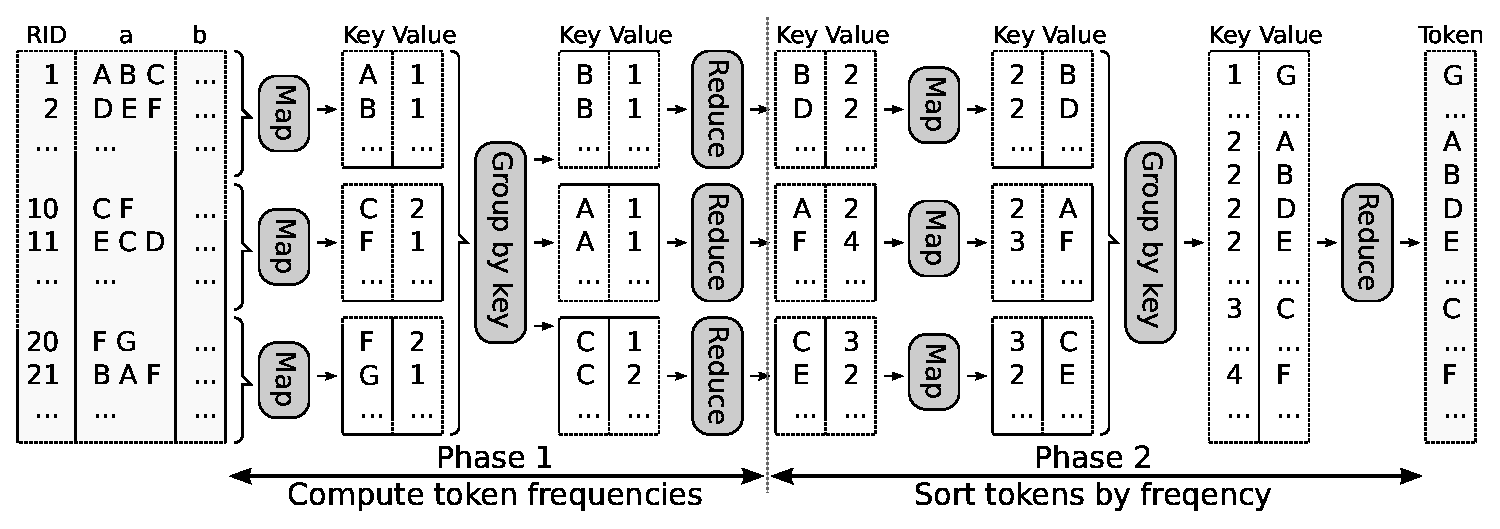
\includegraphics[scale=0.7]{images/fuzzyjoin-tokensbasic}
    \caption{Example data flow of Stage 1 of Set-Similarity
      Joins. (Basic Token ordering for a self-join on attribute
      ``\texttt{a}''.)}
    \label{fig:fuzzyjoin-tokensbasic}
    %% \end{figure}

    %% \begin{figure}
    \center
    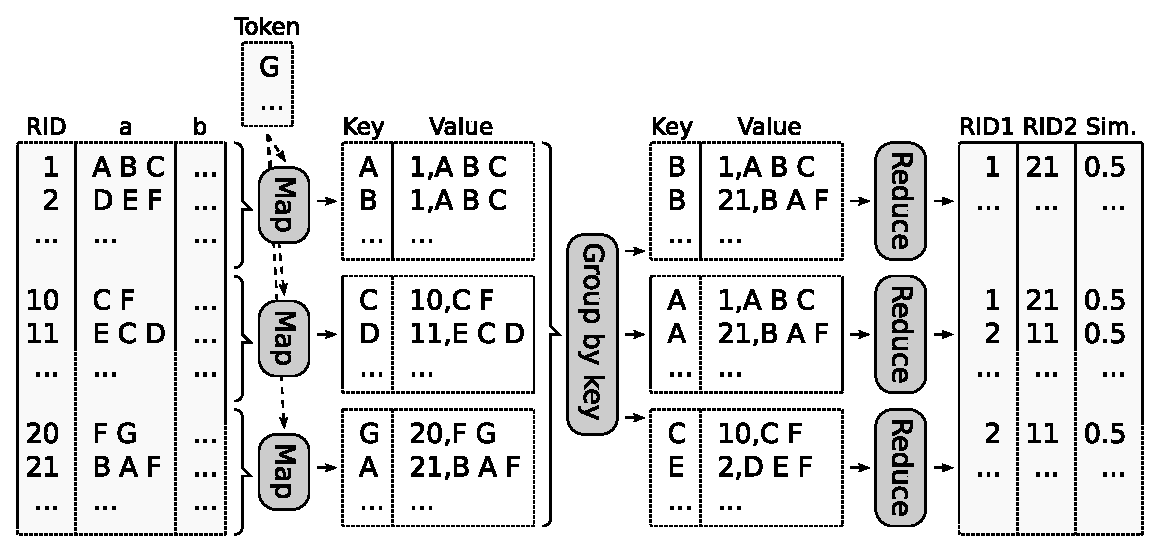
\includegraphics[scale=0.7]{images/fuzzyjoin-ridpairsimproved}
    \caption{Example data flow of Stage 2 of Set-Similarity
      Joins. (Basic Kernel for a self-join on attribute ``\texttt{a}''.)}
    \label{fig:fuzzyjoin-ridparisimporved}
    %% \end{figure}
\end{figure}

    \begin{figure}
    \center
    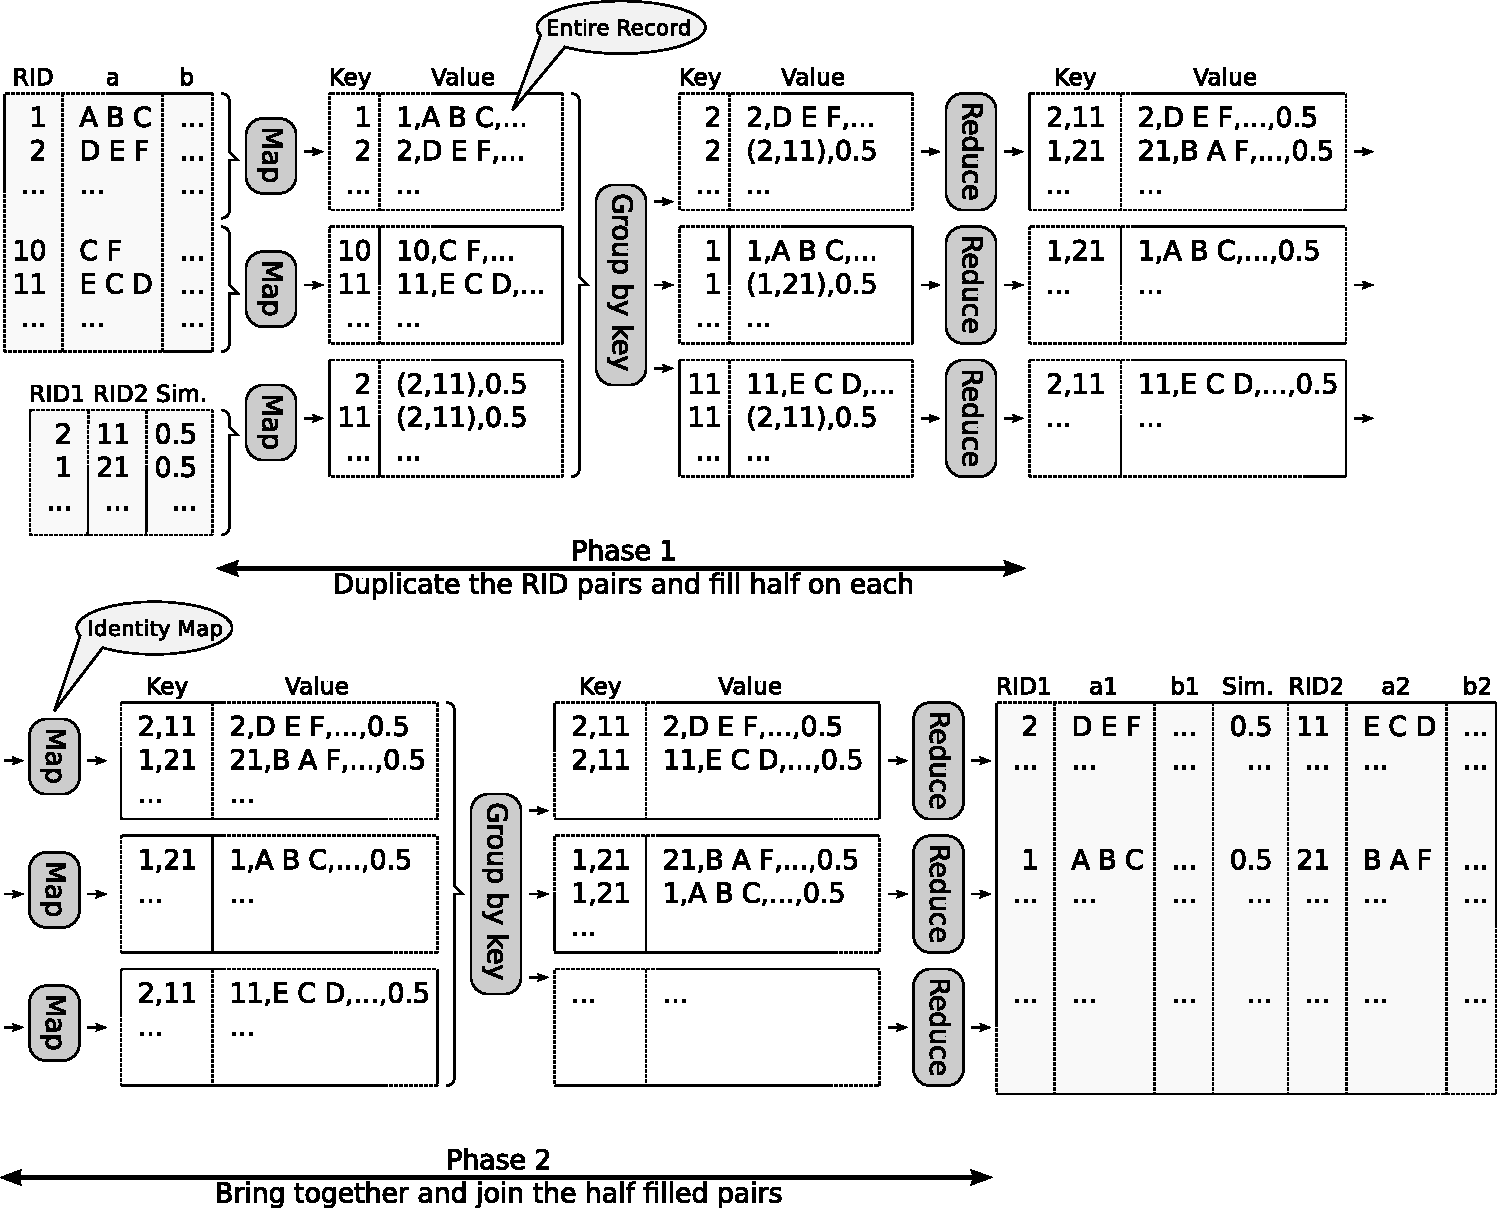
\includegraphics[scale=0.7]{images/fuzzyjoin-recordpairsbasic}
    \caption{Example data flow of Stage 3 of Set-Similarity Joins using
      Basic Record Join for a self-join case. ``\texttt{a1}'' and
      ``\texttt{a2}'' correspond to the original attribute
      ``\texttt{a}'', while ``\texttt{b1}'' and ``\texttt{b2}''
      correspond to attribute ``\texttt{b}''.}
    \label{fig:fuzzyjoin-recordparisbasic}
    \end{figure}
For comparing the performance of Set-Similarity Joins (SSJ), we used the algorithm shown in the figures to find publications with similar titles in the DBLP
dataset~\cite{dblp:xml} by performing a
join of the DBLP data with itself. In order to test performance for different sizes of data, we increased the DBLP data sizes to 5x, 10x, and 25x over the original dataset
(which contains
approximately 1.2M entries) using the replication scheme of~\cite{FuzzyJoinMR}. Table~\ref{tbl:sizeup-fuzzyjoins} shows the running times for the three
stages of the SSJ algorithm on the three different sizes of data. The row labeled ``Hadoop'' represents the time taken to run each stage as a Hadoop job; ``Compat'' shows the
time taken to run the same MapReduce jobs using the compatibility layer on Hyracks (Please ignore the row labeled ``Native'' for now; it will be explained shortly).

\begin{table} [htb!]
\caption{Size-up for Parallel Set-Similarity Joins (10 nodes)}\label{tbl:sizeup-fuzzyjoins}
\center
\begin{tabular}{cl||c|c|c|c}
                     &        & Stage 1 & Stage 2 & Stage 3 & Total time\\
\hline\hline
\multirow{3}{*}{5x}  & Hadoop &   75.52 &  103.23 &   76.59 &  255.34 \\
                     & Compat &   24.50 &   38.92 &   23.21 &   86.63 \\
                     & Native &    11.41 &   32.69 &    9.33 &   53.43 \\
\hline
\multirow{3}{*}{10x} & Hadoop &   90.52 &  191.16 &  107.14 &  388.82 \\
                     & Compat &   42.15 &  128.86 &   38.47 &  209.49 \\
                     & Native &   16.14 &   81.70 &   14.87 &  112.71 \\
\hline
\multirow{3}{*}{25x} & Hadoop &  139.58 &  606.39 &  266.26 & 1012.23 \\
                     & Compat &  105.98 &  538.74 &   60.62 &  705.34 \\
                     & Native &   34.50 &  329.30 &   27.88 &  391.68 \\
\end{tabular}
\end{table}

In the column labeled ``Stage 1'' in Table~\ref{tbl:sizeup-fuzzyjoins}, we see that the MapReduce jobs running on Hadoop scale smoothly with increasing data sizes.
The Hadoop compatibility layer on Hyracks
also shows this trend. However, the job running on Hyracks is faster because it benefits from two improvements: low job startup overhead and more efficient data movement
by the infrastructure.
Hyracks uses push-based job activation, which introduces very little wait time between the submission of a job by a client and when it begins running on the node controllers.

In the column labeled ``Stage 2'' in Table~\ref{tbl:sizeup-fuzzyjoins}, we observe a near constant difference between the running times of Hadoop and Hyracks. This is because
most of the time in this stage is spent in the Reducer code that uses a quadratic algorithm~\cite{FuzzyJoinMR} to find matching records.
The key thing to note is that
most of
the work in this stage is done in the Reduce phase in user-defined code, so the only improvement we can expect is due to lower overhead of the infrastructure.

The column labeled ``Stage 3'' in Table~\ref{tbl:sizeup-fuzzyjoins}, shows that at 5x data size, the ratio of the Hadoop completion time to the Hyracks compatibility
layer completion time is 3.3; the ratio drops to about 2.8 at the 10x
data size. As the amount of data grows to 25x, we see the compatibility layer completing about 4 times faster than Hadoop.
This is because Stage 3 performs two ``joins'' of the record-ids with the original data to produce similar-record-pairs from the similar-record-id-pairs that were produced by
the previous
stage. Every join step reshuffles all of the original input data from the Map to the Reduce phase, but the output of the join is fairly small. Most of the work is thus
performed in moving the data (as the Map and Reduce code is fairly simple). At smaller data sizes, Hadoop times are dominated by startup overhead, while for larger data
sizes the dominating factor is data redistribution. 

\subsubsection{TPC-H}

The TPC-H query is the query from the Hyracks running example that was introduced in Section~\ref{ch:hyracks:sec:overview:subsec:example}. Figure~\ref{fig:tpchmr} shows the structure of the two
MapReduce jobs corresponding to the running example from Figure~\ref{fig:example01_spec}.

\begin{figure} [htb!]
  \centering
  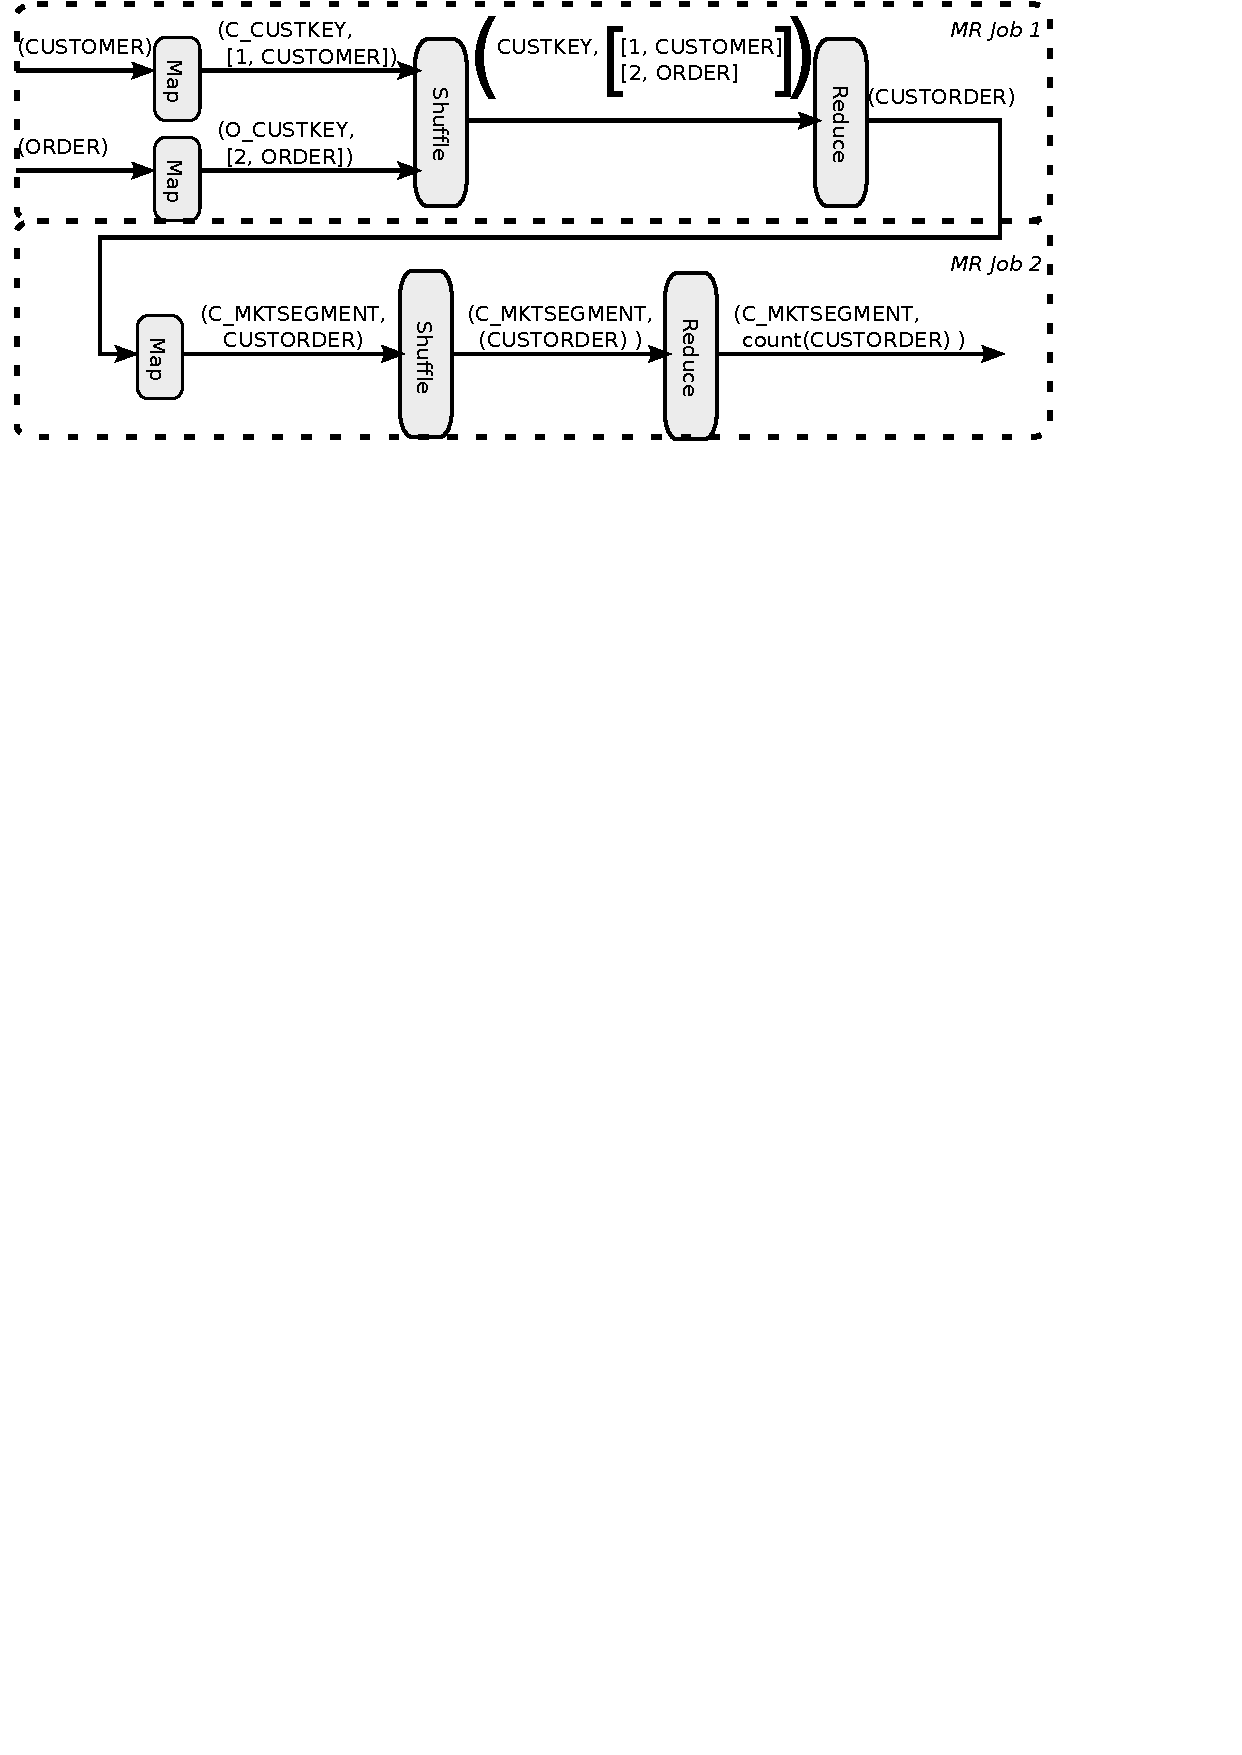
\includegraphics[scale=1]{images/tpch-mr}
  \caption{Hadoop implementation of TPC-H query from Fig.~\ref{fig:example01_spec}.}
  \label{fig:tpchmr}
\end{figure}

The first MapReduce job in Figure~\ref{fig:tpchmr} performs the join using the tagged-join method described in \cite{MapReduceBenchmark}, while the second job computes
the aggregation.  The Mapper of the first job generates the value field as a tagged output that indicates whether the record is
from the CUSTOMER source or the ORDER source. The associated key is generated by extracting the C\_CUSTKEY field if it is a customer record or the O\_CUSTKEY if it
is an ORDER record.
The Reducer of the join job then receives all records (both CUSTOMER and ORDER) that match on the join key. The Reducer function then generates the CUSTOMER-ORDER pairs
to be sent to the output.
The data generated from this first MapReduce job is used as the input for the second MapReduce job, which performs the aggregation step by grouping
the data on the value of the C\_MKTSEGMENT field and then computing the desired count. The Mapper of this job produces the value of C\_MKTSEGMENT as the key and the
CUSTOMER-ORDER pair as the value. The Reducer thus receives
a list of CUSTOMER-ORDER pairs for the same value of C\_MKTSEGMENT that it then counts. The final query output is emitted as a pair of C\_MKTSEGMENT and count values.

As with the other tasks, we measured the end-to-end response time of the jobs by running them on Hadoop and comparing that with the time it took to run the
same MapReduce jobs on Hyracks using the compatibility layer. In addition to the standard configuration of running the two MapReduce jobs sequentially, with HDFS used to store
the intermediate join result, we also executed the compatibility layer with ``pipelining'' between jobs turned on. In this case the join job pipelines data to the aggregation
MapReduce job without the use of HDFS.

As we see from Figure~\ref{fig:tpch-sizeup}, TPC-H on Hadoop takes about 5.5 times the time taken by the compatibility
layer on Hyracks for smaller data sizes (scale 5). Job start-up overhead in Hadoop is responsible for this slowness. As data sizes grow, we observe that the running times for
Hadoop and the compatibility
layer grow super-linearly. This is not surprising since there are two sort steps involved, one in the first MapReduce job to perform the join of CUSTOMER and ORDER data, and
the second to perform aggregation in the second MapReduce job. The result of the join is quite large, and hence a substantial amount of time is spent in partitioning and
sorting. To measure the time spent in writing the join results to HDFS and reading it back in, we also ran in compatibility mode with pipelining turned on. We observe from
Figure~\ref{fig:tpch-sizeup} that I/O to and from HDFS adds significant overhead. At scale 40, the compatibility layer takes about 133 seconds (about 25\% longer
than the pipelined execution).
Note however that all of the MapReduce running times exhibit a super-linear curve owing to the sort operations (We will ignore the ``Hyracks Native'' curve for now).

\begin{figure} [htb!]
  \centering
  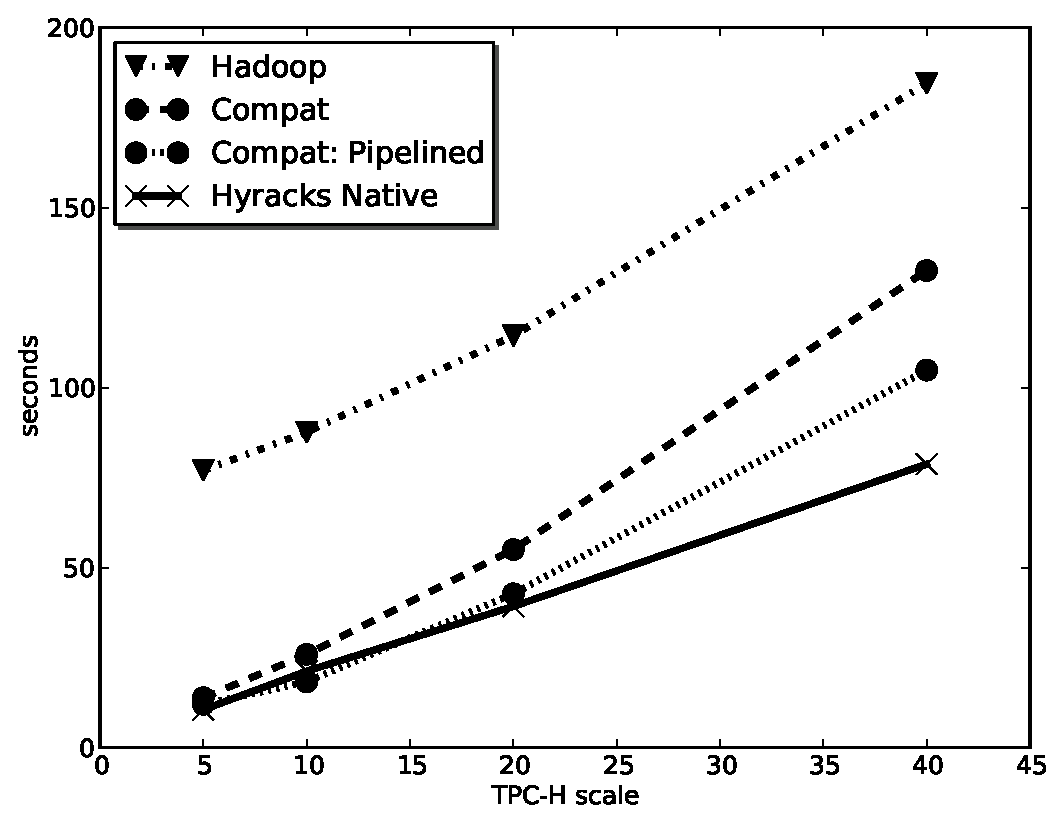
\includegraphics[scale=0.6]{images/tpch-sizeup}
  \caption{TPC-H query from Fig.~\ref{fig:example01_spec} with Hadoop and Hyracks.}
  \label{fig:tpch-sizeup}
\end{figure}

\subsection{Beyond MapReduce}

We now show the results of running two experiments to study the performance improvements obtainable in Hyracks by not being restricted to the MapReduce programming model.
We present results for Set-Similarity Joins and the TPC-H join/aggregate example query.

\subsubsection{Set-Similarity Joins (Take 2)}

\begin{figure} [htb!]
    %% \begin{figure}
    \center
    \includegraphics[scale=0.5]{images/fuzzyjoin-hyrax-stage1}
    \caption{Hyracks-native plan for Stage 1 of Set-Similarity Self-Joins.}
    \label{fig:fuzzyjoin-hyrax-stage1}
    %% \end{figure}
    %% \begin{figure}
    \center
    \vspace{.5em}
    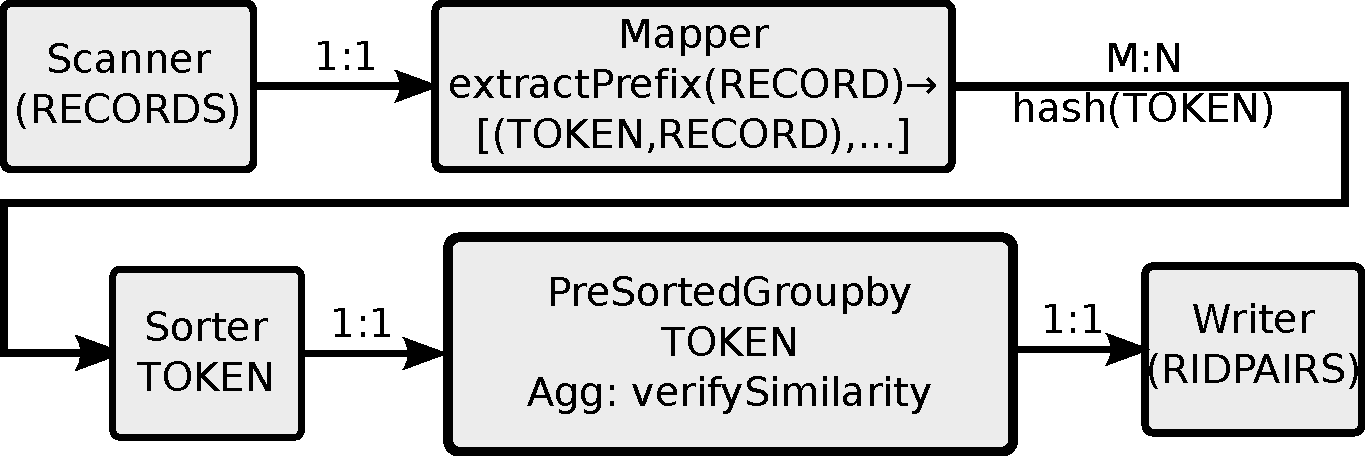
\includegraphics[scale=0.5]{images/fuzzyjoin-hyrax-stage2}
    \caption{Hyracks-native plan for Stage 2 of Set-Similarity Self-Joins.}
    \label{fig:fuzzyjoin-hyrax-stage2}
    %% \end{figure}
    %% \begin{figure}
    \center
    \vspace{.5em}
    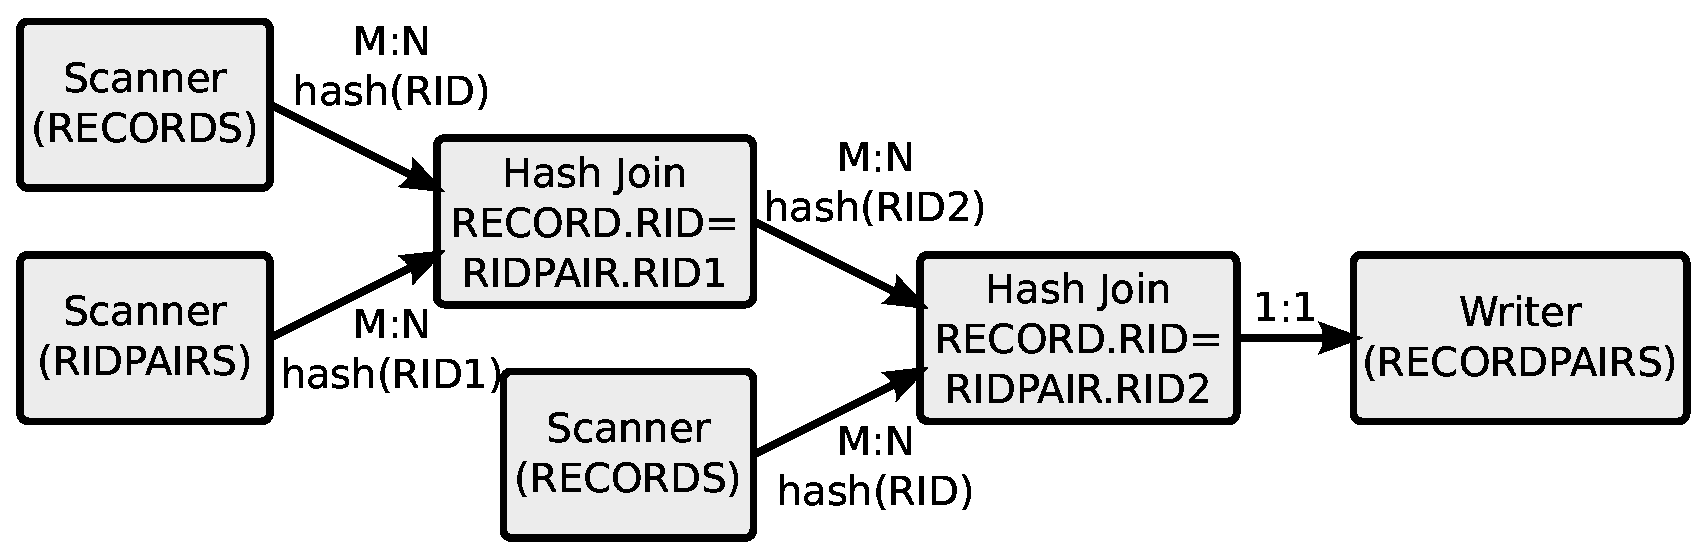
\includegraphics[scale=0.5]{images/fuzzyjoin-hyrax-stage3}
    \caption{Hyracks-native plan for Stage 3 of Set-Similarity Self-Joins.}
    \label{fig:fuzzyjoin-hyrax-stage3}
    %% \end{figure}
\end{figure}

Figures \ref{fig:fuzzyjoin-hyrax-stage1}, \ref{fig:fuzzyjoin-hyrax-stage2}, and \ref{fig:fuzzyjoin-hyrax-stage3} show the native Hyracks job specifications to
implement the three stages of the Hadoop based Set-Similarity Join examined in the previous subsection.

In Table~\ref{tbl:sizeup-fuzzyjoins}, the row labeled ``Native'' shows the time
required by the Hyracks jobs to perform Set-Similarity Joins. We can now compare these
times to those that we examined previously. These faster Native times are due in part to the savings
already discussed, but here we also see additional algorithmic benefits. Stage 1 benefits the most
from the Native formulation due to the use of hash based grouping, which does not need
to sort the input data like in Hadoop. Stage 3, in the Native case, benefits from using
hash join operators that perform the joins by building a hash-table on one of their inputs
and then probing the table using the other input. This strategy is cheaper than first
sorting both inputs on the join key to bring the matching values from both the sides
together (which is what happens in Hadoop). In Stage 2, we used sort-based grouping since it performed
slightly better than its hash-based counterpart. Usually, hash-based aggregation works well
for traditional aggregates when grouping is performed on relatively low cardinality attributes, as
compression is achieved by the aggregation. In the case of Stage 2, however, the grouping
operation is used to separate the input into groups without applying an incremental aggregation function.
The sort operator in Hyracks implements the ``Poor man's normalized key'' optimization mentioned
in~\cite{GraefeCPUCache} which can be exploited when building Hyracks Native jobs.
This optimization helps in terms of providing cheaper comparisons and better cache locality.  
After sorting, the ``aggregation'' function performs a quadratic scan of the items
within each group. This is seen in Table~\ref{tbl:sizeup-fuzzyjoins} as a super-linear growth in the completion time for Stage 2.

In summary, we see that the Native formulation of Set-Similarity Joins run about 2.6 to 4.7
times faster than their MapReduce formulation running on Hadoop and about 1.6 to 1.8
times faster than running the same MapReduce jobs on Hyracks using its compatibility layer.

\subsubsection{TPC-H (Take 2)}

We now compare the two MapReduce TPC-H implementations with the native Hyracks implementation.
The ``Hyracks Native'' line in Figure~\ref{fig:tpch-sizeup} shows the results of natively running the TPC-H query in Figure~\ref{fig:example01_spec}.
Notice that for large data the TPC-H query executes on Hyracks much faster than the MapReduce counterparts on Hadoop or on Hyracks via the compatibility layer. As in the
native expression of
Set-Similarity Joins, this is due in part to the fact that the TPC-H query uses hash-joins and hash-based aggregation. In addition, Hyracks does not need to materialize
intermediate results between the
joiner and the aggregator. In contrast, since Hadoop accepts one MapReduce job at a time, it needs to persist the output of the Join job for this example in HDFS. To
minimize the ``damage'' caused by this materialization on the Hadoop completion time, we set the replication factor in HDFS to 1 (meaning no replication). We observe that
the Hyracks job scales linearly with growing data size since all operations in the pipeline have linear computational complexity for the memory and data sizes
considered here.

To conclude, Hyracks is a more efficient alternative to Hadoop for MapReduce jobs, and even greater performance benefits can be achieved by not being restricted
to the MapReduce programming model. Here we have compared the performance characteristics of Hadoop and Hyracks in detail for K-Means clustering, Set-Similarity joins, and an
example TPC-H query. We have measured even greater benefits for simpler jobs. For example, the standard Hadoop Word-Count MapReduce job on 12 GB of data ran approximately twice
as fast on Hyracks using the compatibility layer than on Hadoop, and a Native Word-Count implementation on Hyracks ran approximately 16 times as fast as the Hadoop
MapReduce version.

\subsection{Fault Tolerance Study}

A system designed to run on a large number of commodity computers must be capable of detecting and reacting to possible faults that might occur during its regular operation.
In this part of the thesis, we perform a very simple experiment to illustrate the fact that, while being able to run jobs through to the end despite failures is valuable,
doing so by being pessimistic and ever-prepared for incremental forward-recovery is not a general ``right'' answer. Hadoop uses a naive strategy based on storing all
intermediate
results to durable storage before making progress. While such a naive strategy is a safe first approach, we wish to begin exploring the path of applying more
selective fault-tolerance. Hyracks is in a better position to exploit operator and connector properties to achieve the same degree of fault tolerance while doing less
work along the way. As our first step in this direction, the Hyracks fault-tolerance strategy that we use for the experiment in this section is to simply restart
all jobs impacted by failures.
Although such a strategy cannot be the only one in a system like Hyracks, we believe that this is actually an effective strategy for smaller to medium-sized jobs.

We used the TPC-H example query shown in Figure~\ref{fig:example01_spec} on data scale 40 for this experiment. In our experimental
set-up, we had the client submit the same job
request over and over again in an infinite loop without any think time and we measured the observed completion time for every request.
Separately, we killed a randomly chosen cluster
node at regular intervals. In different runs of the experiment, we changed the mean time between failures from 100 seconds to 1600 seconds. The same experiment was
performed with the jobs running on Hyracks and then with the corresponding jobs running on Hadoop. Figure~\ref{fig:tpch-fault-tolerance} shows the observed request
completion time (retry times included) for the two systems for different MTBF (mean time between failure) values. The data inputs to the jobs in both systems were
replicated so that a node failure could still allow progress of the job.

\begin{figure} [htb!]
  \centering
  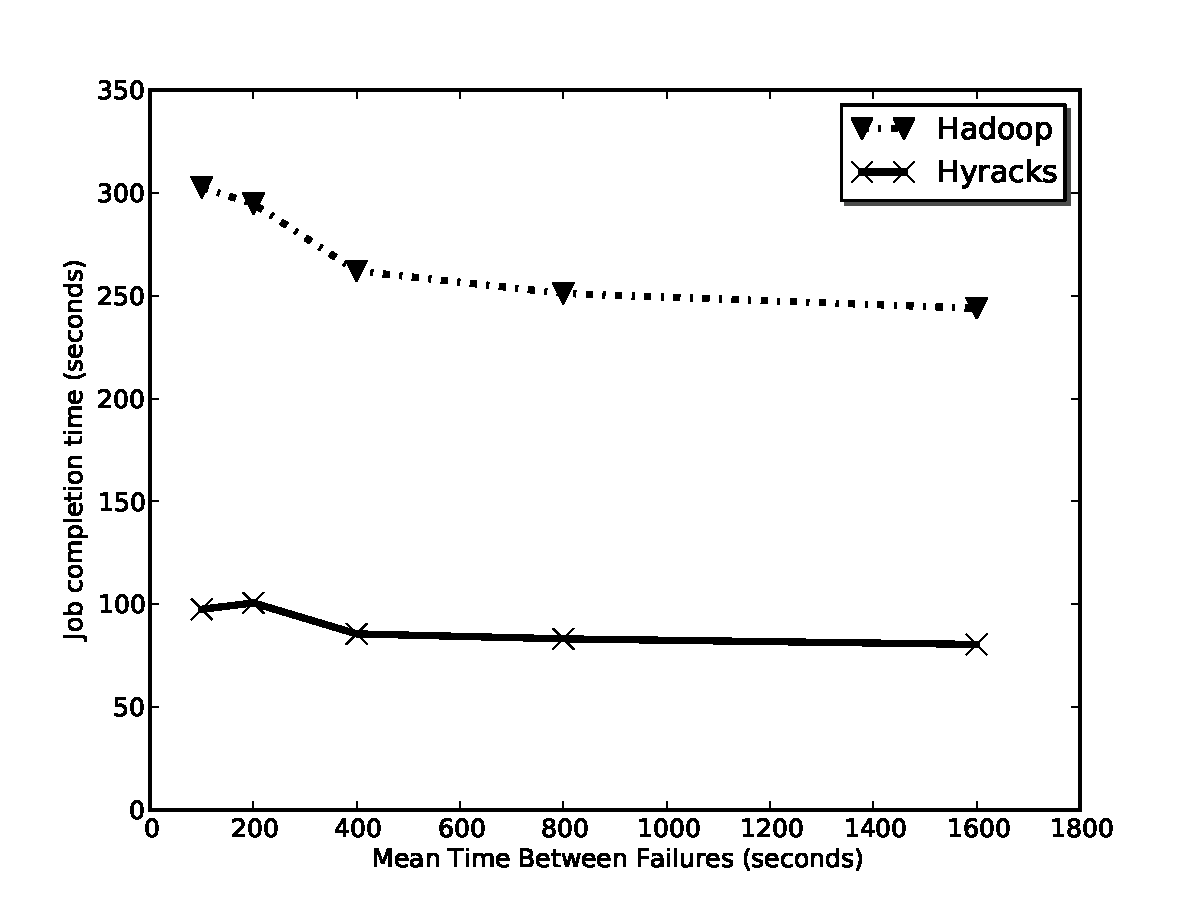
\includegraphics[scale=0.6]{images/tpch-fault-tolerance}
  \caption{TPC-H query from Fig.~\ref{fig:example01_spec} in the presence of failures.}
  \label{fig:tpch-fault-tolerance}
\end{figure}

In Hadoop in order to provide as much isolation from failures as possible, every
map task writes its output to the local disk before its data is made available to the reducer side. On the reducer side, every partition fetched from every map task is written
to local disk before a merge is performed. The goal of the extra I/O in Hadoop is to make sure that at most one task needs to be restarted when a failure occurs. In the current
implementation of Hyracks, however, data is pipelined from producers to consumers, so a single failure of any one node requires a restart of all of the operators that are 
currently part of the same pipelined stage.

We observe from Figure~\ref{fig:tpch-fault-tolerance} that Hyracks runs the TPC-H job to completion faster even when failures are injected into the cluster very frequently.
Note also that, since a given Hyracks job runs to completion much faster than the ``fault-tolerant'' Hadoop job, a given Hyracks job is less likely to be hit by a failure
during its execution in the first place.

As we mentioned earlier, a strategy
that requires a complete restart cannot be the only fault recovery strategy in a system. If the mean time between failures is less than the mean time to complete a
job, then such a job
may never complete.

\section{Conclusion}

This chapter described the design and implementation of Hyracks. Hyracks was built from the group-up to serve as an efficient, parallel, dataflow runtime platform. Based on the the performance comparison performed with the Hadoop MapReduce layer for a variety of tasks, we can conclude that the design philosophy of Hyracks has merit. Since its availability as an open-source project, Hyracks has also proven to be a successful research platform that has been used to build various other systems on top of. For example, Hyracks has been used to build the Pregelix layer to perform graph analytics at massive scale, which in turn has been used to solve graph problems arising in the field of genetics.
